\documentclass[parskip=half,final,oneside,a4paper]{scrartcl}

\usepackage[final]{microtype}
\usepackage{lmodern}
\usepackage{tikz}
\usepackage{graphicx}
\usepackage[utf8]{inputenc}
\usepackage[T1]{fontenc}
\usepackage{marvosym}
\DeclareUnicodeCharacter{20AC}{\EUR{}}
\usepackage{xcolor}
\usepackage{moresize}
\usepackage{tabularx}
\usepackage{siunitx}
\usepackage{multicol}

\DeclareSIUnit{\euro}{\text{\EUR{}}}

\usetikzlibrary{calc,fit,backgrounds}

\usepackage[disable,colorinlistoftodos]{todonotes}


\usepackage[%
        pdftitle={GUADEC 2016 Bid for Karlsruhe},
        pdfauthor={},
        pdfsubject={GUADEC 2016 Bid},
        pdfkeywords={GUADEC, 2016, Bid},
        bookmarksopen=true,
        pdfpagemode=UseOutlines,
        pdfdisplaydoctitle=true,
        pdfview=FitH,
        pdfpagelayout=TwoColumnRight,
        pdflang=en,
        breaklinks=true
]{hyperref}


\KOMAoptions{DIV=last}


\author{Moira Schuller, Benjamin Berg, Tobias Müller, Markus Morhard}
\title{2016 -- Bid Karlsruhe}

\newcounter{imgnumber}
\setcounter{imgnumber}{1}

\makeatletter

\def\imagecopyrights{}

%\setlength{\parindent}{0pt}
\newcommand\imgtitle[3]{ %
  Image \#\theimgnumber{}, #2 %
%
  \g@addto@macro{\imagecopyrights}{\item #2, #1, #3}%
%
  \addtocounter{imgnumber}{1}%
}

\makeatother



\begin{document}

  \thispagestyle{empty}

  \begin{tikzpicture}[remember picture,overlay]
    \node[anchor=north,yshift=-5cm,text width=0.7\linewidth] at (current page.north) {
      \begin{center}
        
\includegraphics{images/guadec-logo.pdf} \\[2em]
        {\sf \HUGE 2016} \\[5em]
        {\sf \Huge Karlsruhe, Germany}
      \end{center}
    };

    \node[anchor=south west,outer sep=0,inner sep=0] (title-img) at (current page.south west) {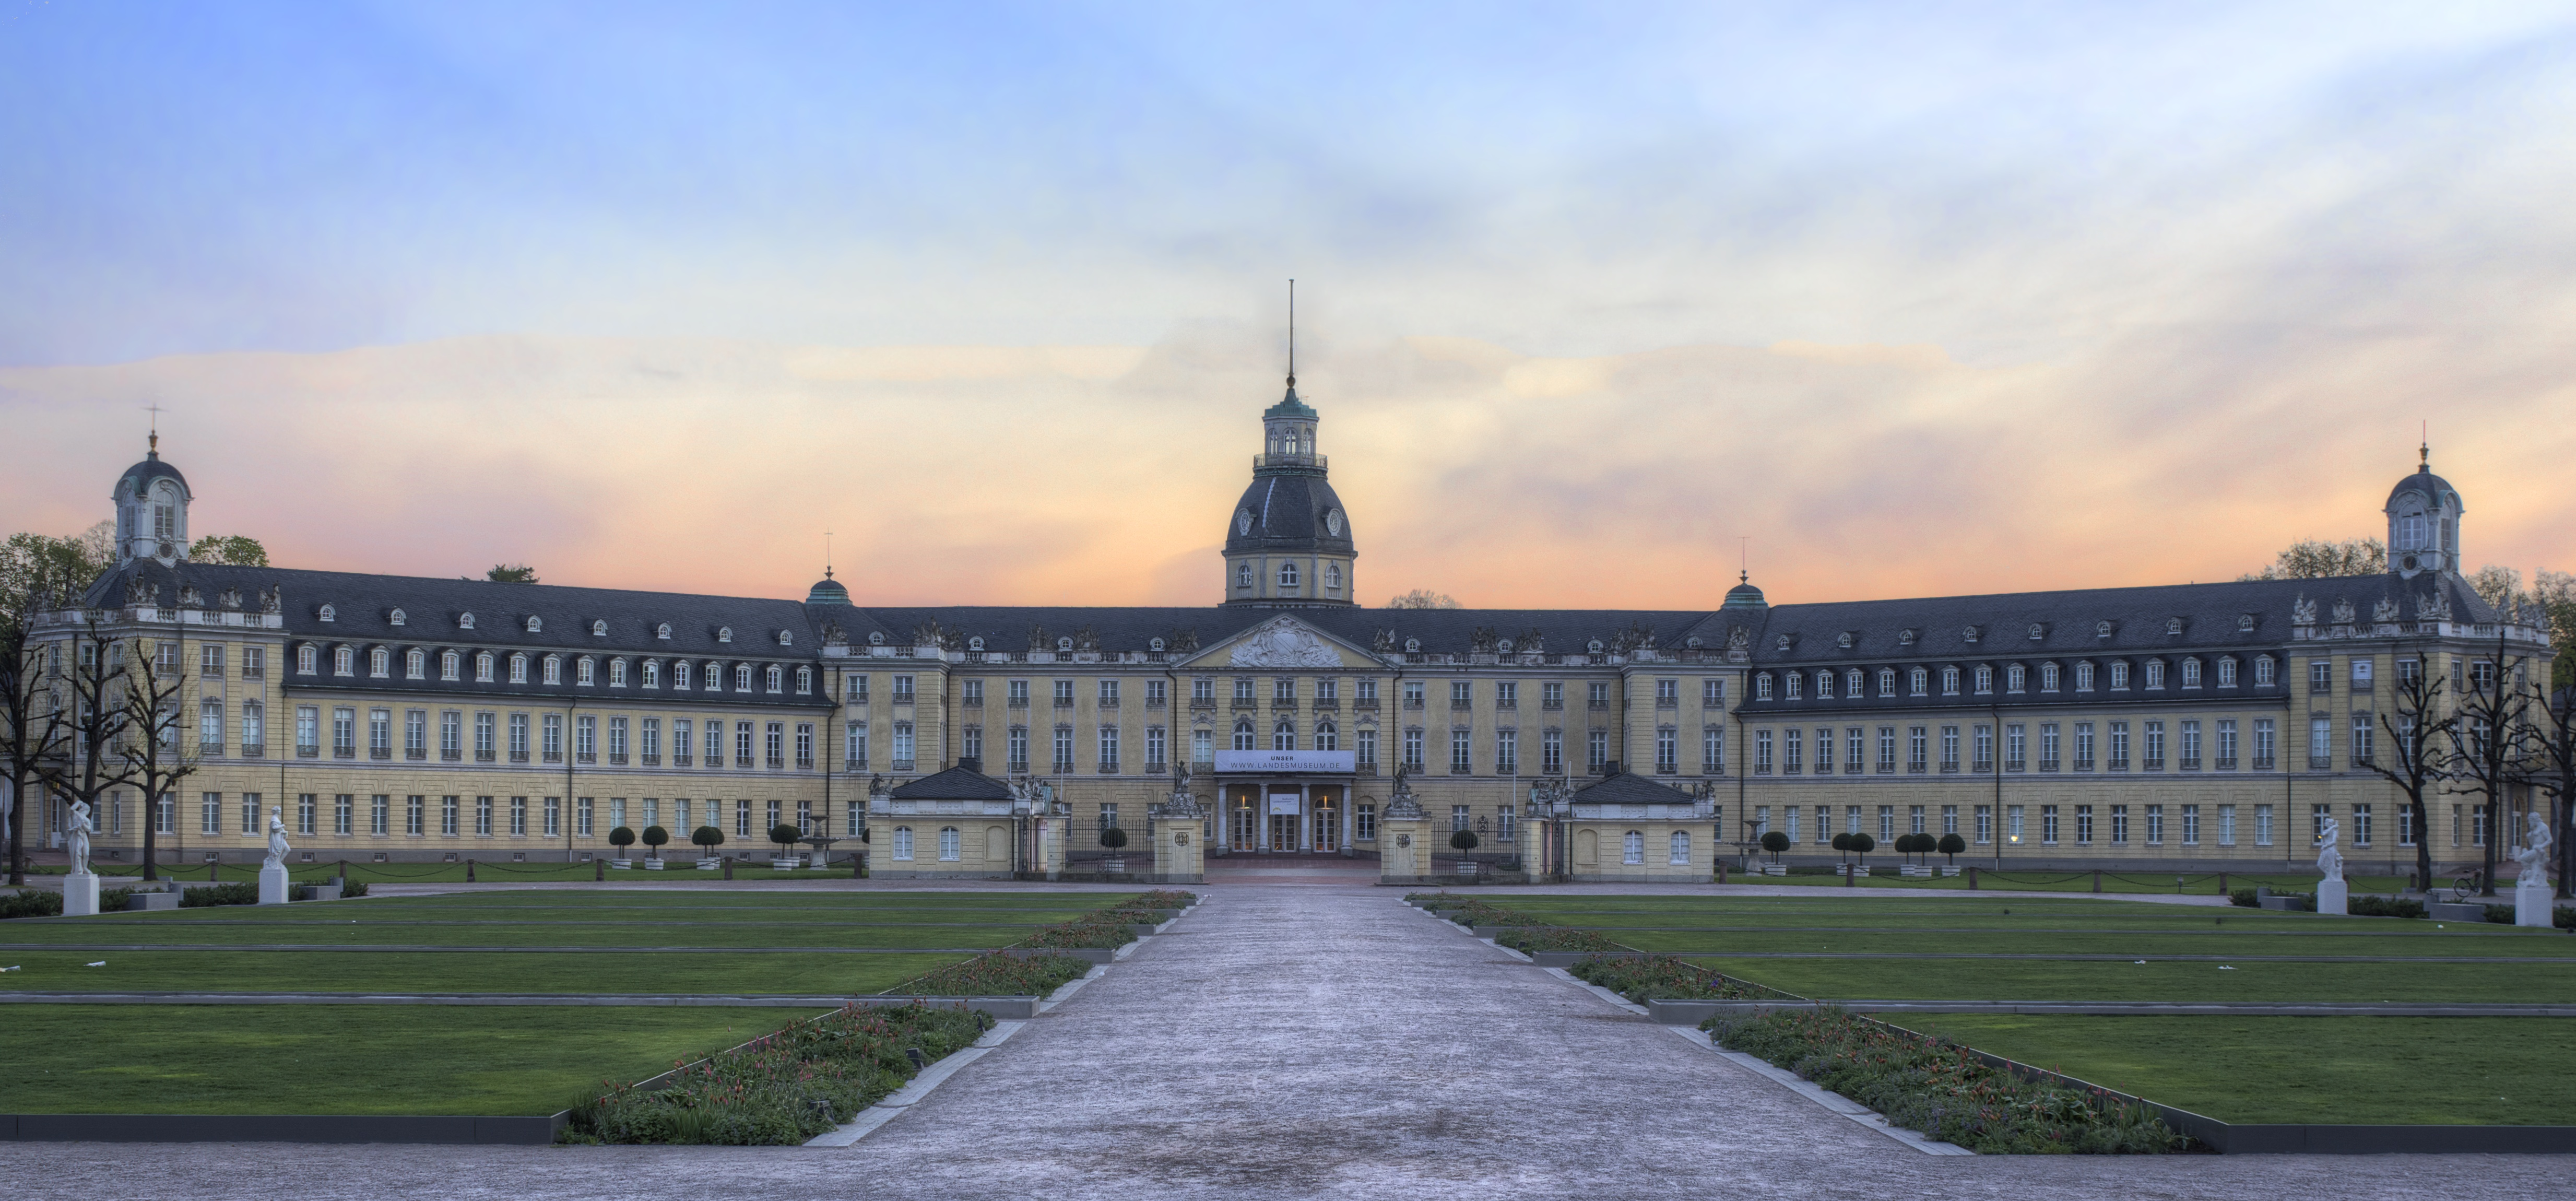
\includegraphics[width=21cm]{images/city/palace-1.jpg}};
    \node[anchor=south west,color=white] at (title-img.south west) {\imgtitle{Christian Reimer}{Karlsruhe Palace}{CC BY-SA 2.0, original title “Karlsruher Schloss on Fire - oder so.”, not modified, \url{https://www.flickr.com/photos/christianreimer/}}};

  \end{tikzpicture}


\newpage

\tableofcontents

\newpage

%%%%%%%%%%%%%%%%%%%%%%%%

\section{Introductory paragraph about the location}

Let's start out with some trivialities that might convince you all that 
hosting GUADEC in Karlsruhe in 2016 is a brilliant idea. Karlsruhe is 
Germany's sunniest city. Karlsruhe is situated in the Southern part of 
Germany, hence not only easily accessible from other European 
Countries, but also from abroad as it is close enough to Frankfurt 
international airport and Stuttgart airport. Karlsruhe combines a 
strong sense for science and technology - think KIT\footnote{Karlsruhe 
Institute of Technology}, FZI\footnote{Forschungszentrum Informatik} 
and Frauenhofer Institute–with a penchant for creativity and 
design–think ZKM\footnote{Zentrum für Kunst und Medien}. Karlsruhe is a 
typical “student city” with affordable accommodation and cheap meals. 
The city hosts 4 higher education institutes offering computer science 
related degrees. As we plan a particular student pre-event to tap into 
this student pool, the potential of growing the GNOME community is 
guaranteed.

%Karlsruhe is the perfect place to host GUADEC 2016.

% Place map on bottom of the page.
\vfill
% getikz enable true
%! Available geTikZ-commands:
% getikz library calc,fit,backgrounds
%! % getikz header <header e.g. \usepackage commands>
% getikz path ../..
%! For a description of these and other commands have a look at
%! https://gitorious.org/getikz/pages/Commands

\def\venue{red}
\def\social{blue}
\def\location#1#2{\draw[line width=2,color=#2,opacity=0.7] (#1) circle[radius=0.025]; }
\def\loclabel#1#2#3{\node[anchor=#1,outer sep=6,fill=white,fill opacity=0.5,text opacity=1,rounded corners] at (#2) {\bf #3}; }

\ifx\imgtitle\undefined
\def\imgtitle#1#2#3{}
\fi

\begin{tikzpicture}

  % 21cm
  \pgfmathsetmacro{\scale}{\linewidth/1190bp}
  \pgfmathsetmacro{\backscale}{1190bp/\linewidth}

  \begin{scope}[scale=\scale]

    % 1190bp scaled manually
    \begin{scope}[on background layer]
      \node[outer sep=0,inner sep=0] (map) {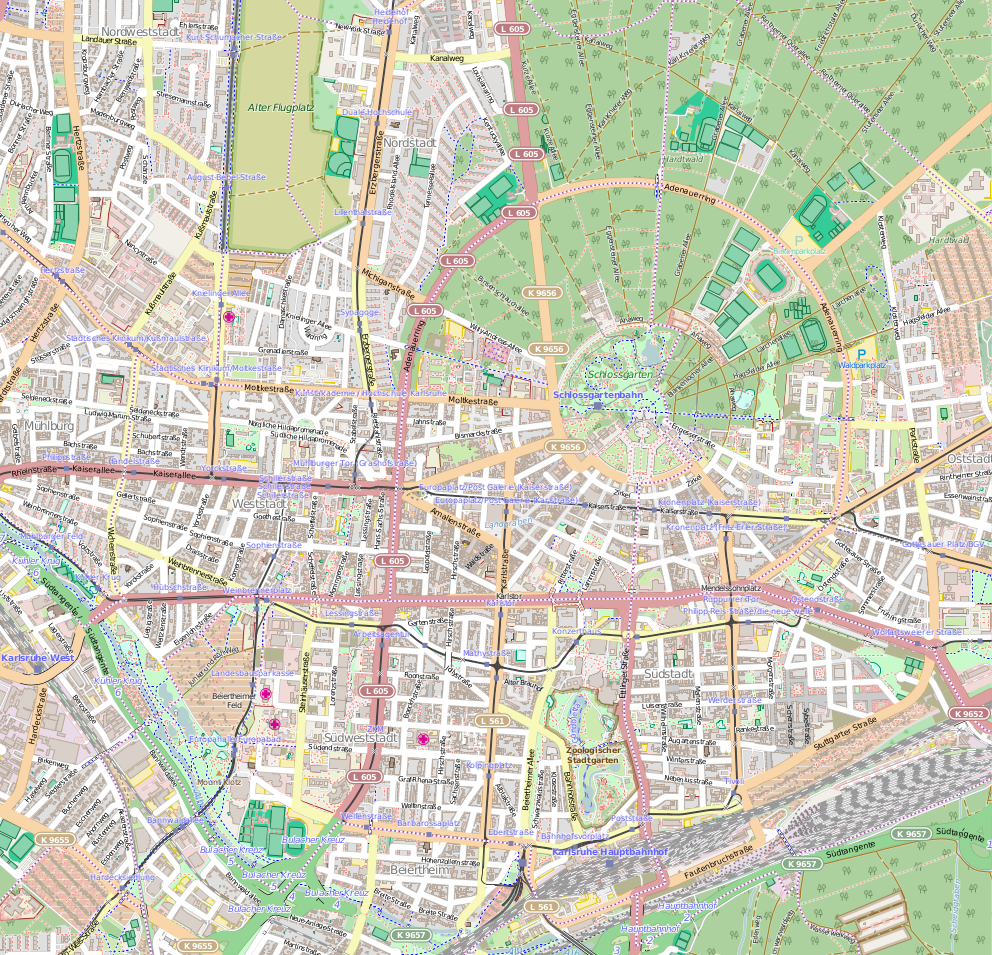
\includegraphics[width=\linewidth,trim=0 100 0 100,clip]{images/map/osm-ka-low.png}};
    \end{scope}

    \node[anchor=center,coordinate] (center) at (6.28cm,2.78cm) {};
    \node[anchor=center,coordinate] (615m) at (14.85cm,2.78cm) {};

    \begin{scope}[shift=(center),scale=1000*(14.85-6.28)/615]
      \node[anchor=center,coordinate] (schloss) at (0,0) {};
      \node[anchor=center,coordinate] (zoo) at (-0.19,-0.95) {};
      \node[anchor=center,coordinate] (hbf) at (-0.2,-1.33) {};
      \node[anchor=center,coordinate] (zkm) at (-0.9,-0.88) {};
      \node[anchor=center,coordinate] (dhbw) at (-0.84,+0.88) {};
      \node[anchor=center,coordinate] (campus) at (+0.35,-0.2) {};
      \node[anchor=center,coordinate] (waldparkplatz) at (+0.68,+0.18) {};
      \node[anchor=center,coordinate] (karlshs) at (-0.46,-0.5) {};
      \node[anchor=center,coordinate] (z10) at (+0.46,-0.36) {};
      \node[anchor=center,coordinate] (akk) at (+0.45,-0.2) {};
      \node[anchor=center,coordinate] (hadiko) at (+0.82,0.4) {};
      \node[anchor=center,coordinate] (jugendherberge) at (-0.5,+0.1) {};
      \node[anchor=center,coordinate] (info) at (+0.68,+0.0) {};
      \node[anchor=center,coordinate] (markt) at (-0.02,-0.3) {};

      \location{schloss}{\social}
      \loclabel{south}{schloss}{Castle and Parc}
      \location{zkm}{\venue}
      \loclabel{east}{zkm}{ZKM}
      \location{karlshs}{\venue}
      \loclabel{north}{karlshs}{Karlshochschule}
      \location{campus}{\venue}
      \loclabel{south}{campus}{KIT/University}
      \location{dhbw}{\venue}
      \loclabel{west}{dhbw}{DHBW}
      \location{z10}{\social}
      \loclabel{north}{z10}{Z10}
      \location{akk}{\social}
      \loclabel{west}{akk}{AKK}
      \location{jugendherberge}{\social}
      \loclabel{north}{jugendherberge}{Youth Hostel}

      %\location{zoo}{\social}
      %\loclabel{east}{zoo}{Zoo}

      \location{markt}{\social}
      \loclabel{north}{markt}{City Center}

      \location{info}{\venue}
      \loclabel{south}{info}{CS Department}

      \location{hbf}{\social}
      \loclabel{south}{hbf}{Main Station}



      \node[coordinate] (legend) at ($(map.south west)+\scale*(2ex, 1.8em)$) {};
      \node[coordinate] (legend-out) at ($(legend)+(1,0)$) {};

      \begin{scope}
        \draw[line width=2pt,opacity=0.7,line cap=round] ($(legend) + (0, 0.025)$) -- (legend) -- node[above,opacity=1,inner sep=0,yshift=2pt] (kmlabel) {1\,km} ++(1, 0) -- ++(0, 0.025);

        \node[anchor=south west,inner sep=0pt] (copyright) at ($(legend) + \scale*(0, -1em)$) {\imgtitle{OpenStreetMap contributors}{Map of Karlsruhe}{CC BY-SA 2.0, overlays added, \url{http://www.openstreetmap.org/copyright}}};
      \end{scope}

      \begin{scope}[on background layer]
        \node[fit=(legend) (legend-out) (kmlabel) (copyright),fill=white,opacity=0.8,rounded corners] {};
      \end{scope}

    \end{scope}
  \end{scope}

\end{tikzpicture}




\section{Venue}

At this point the most promising option that we have is the Duale Hochschule
Baden-Württemberg (DHBW). We are however still in investigating other options
at this point.

\subsection{DHBW}

\begin{tikzpicture}
  \begin{scope}[on background layer]
    \node[inner sep=0,outer sep=0] (main) {%
      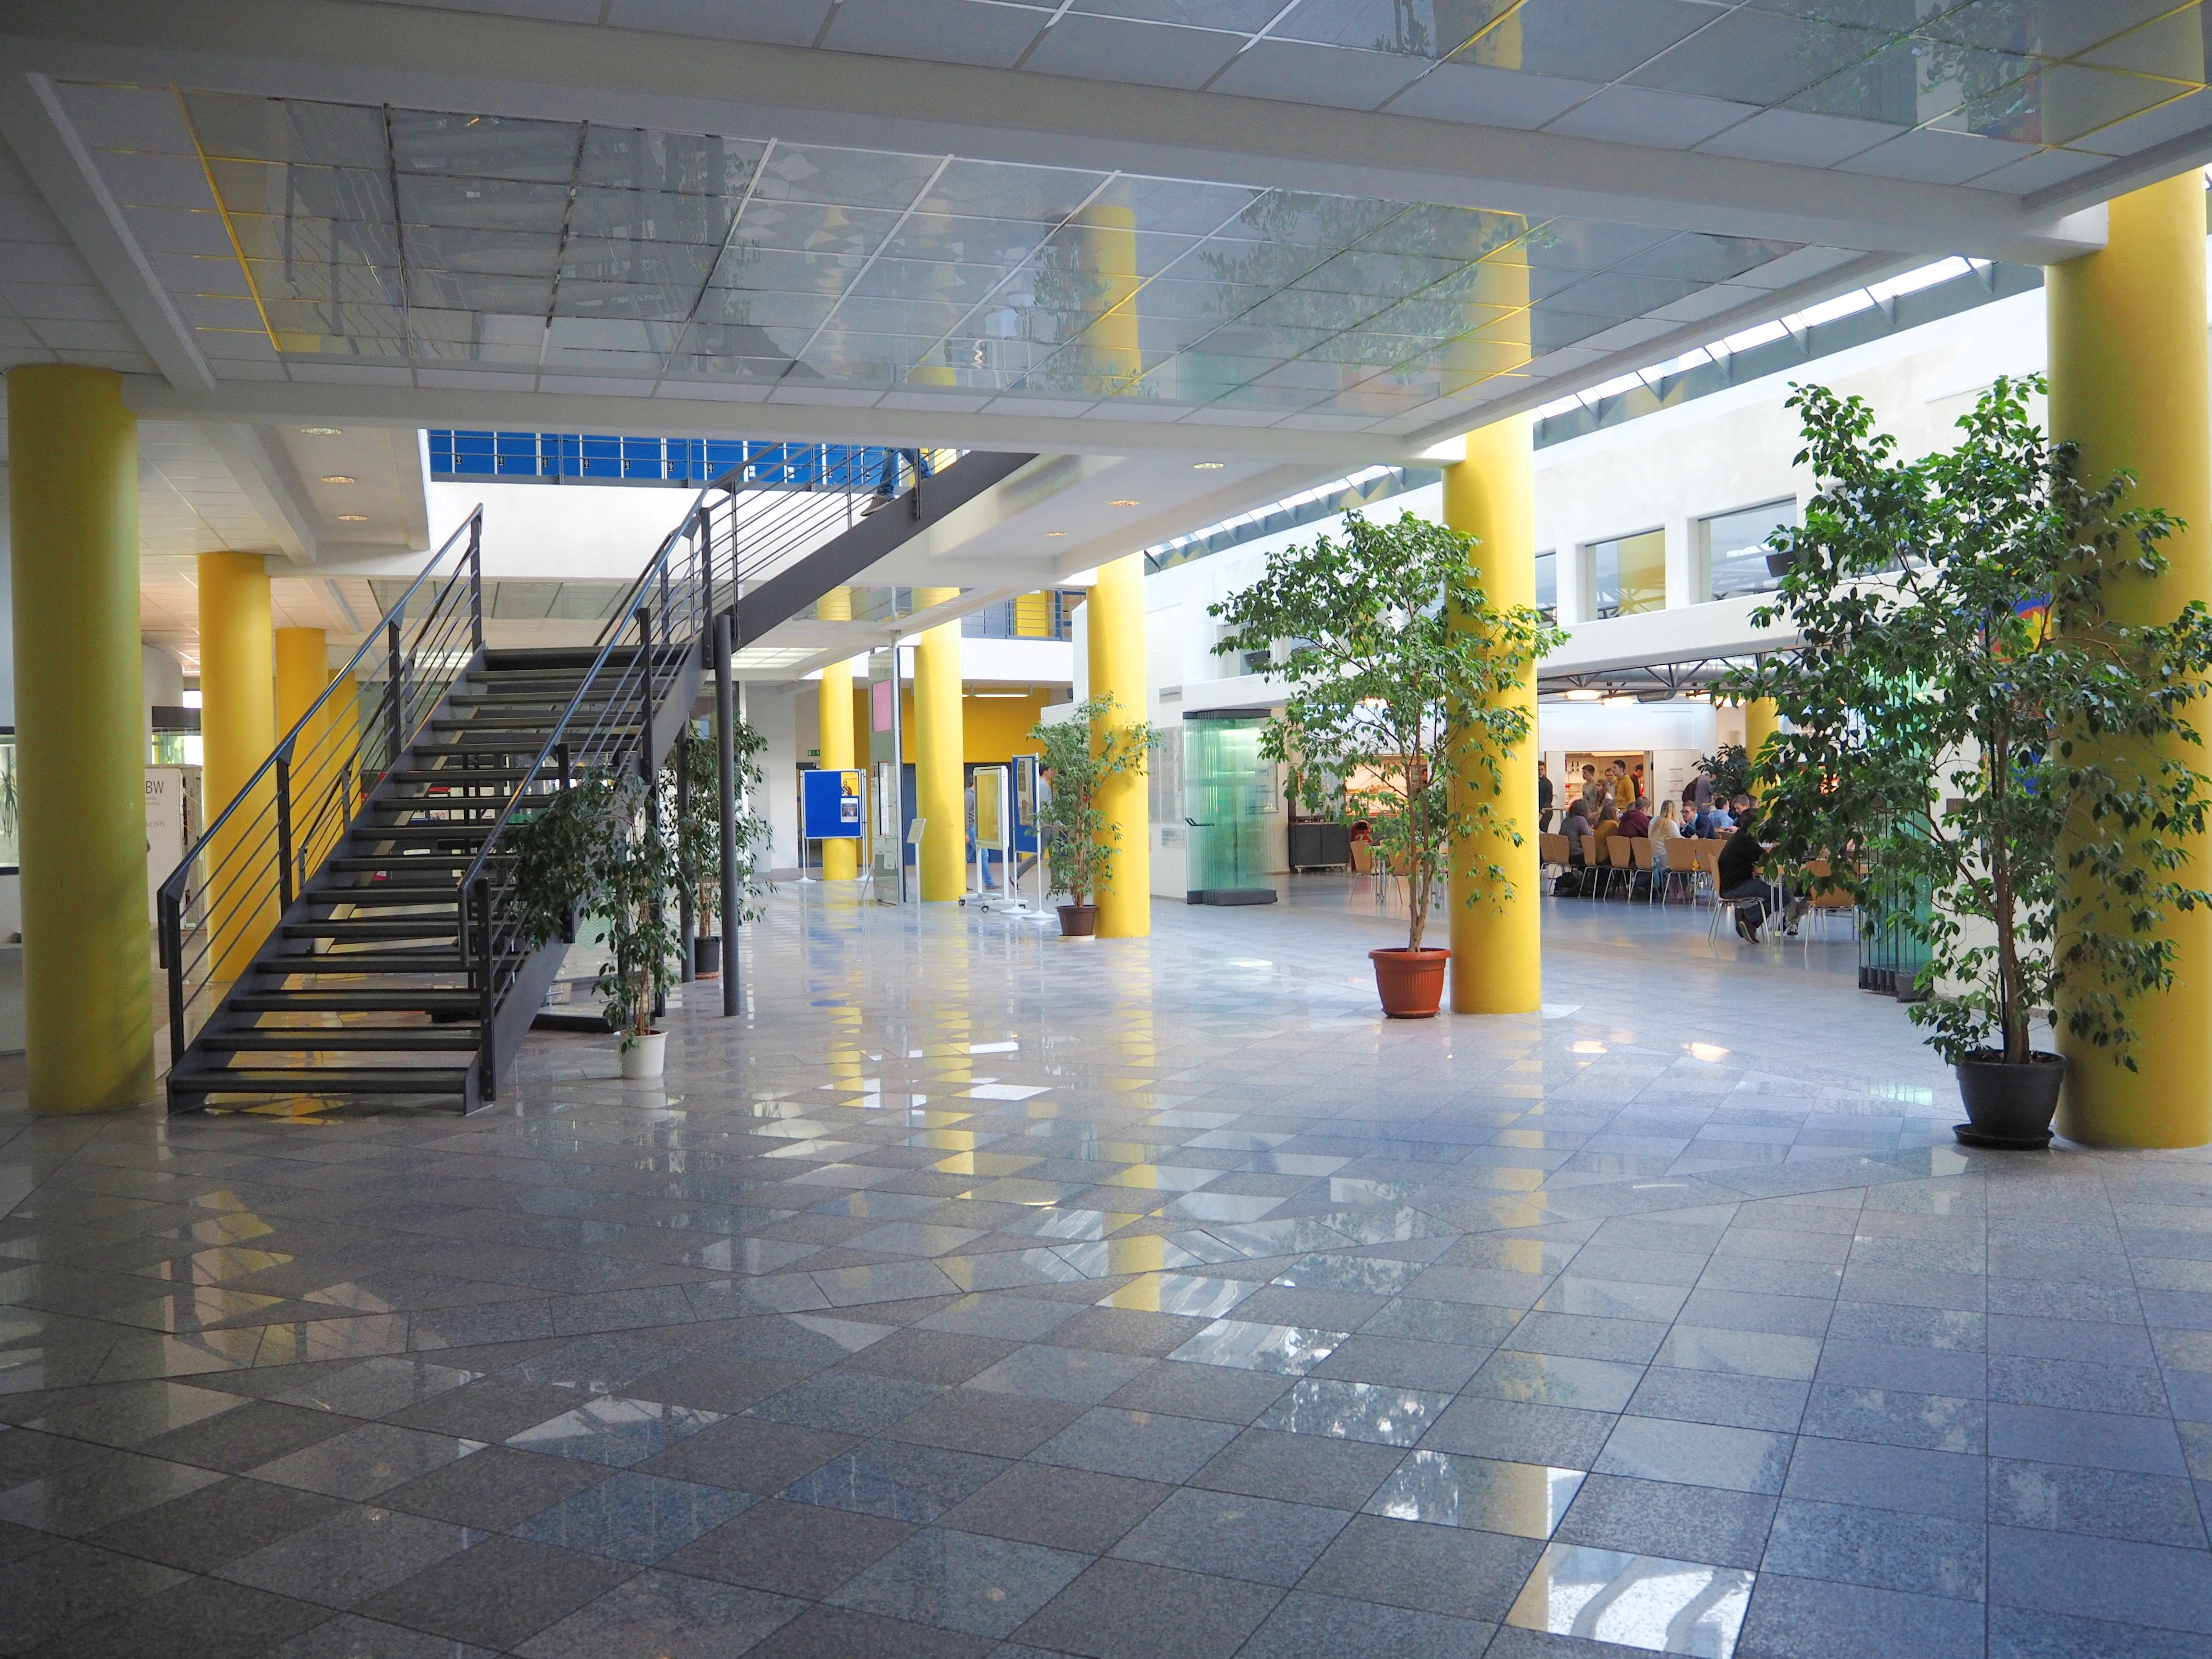
\includegraphics[width=0.5\linewidth]{images/venues/dhbw/P9280379}%
    };
    \node[inner sep=0,outer sep=0,anchor=north west] (sub-1) at (main.north east) {%
      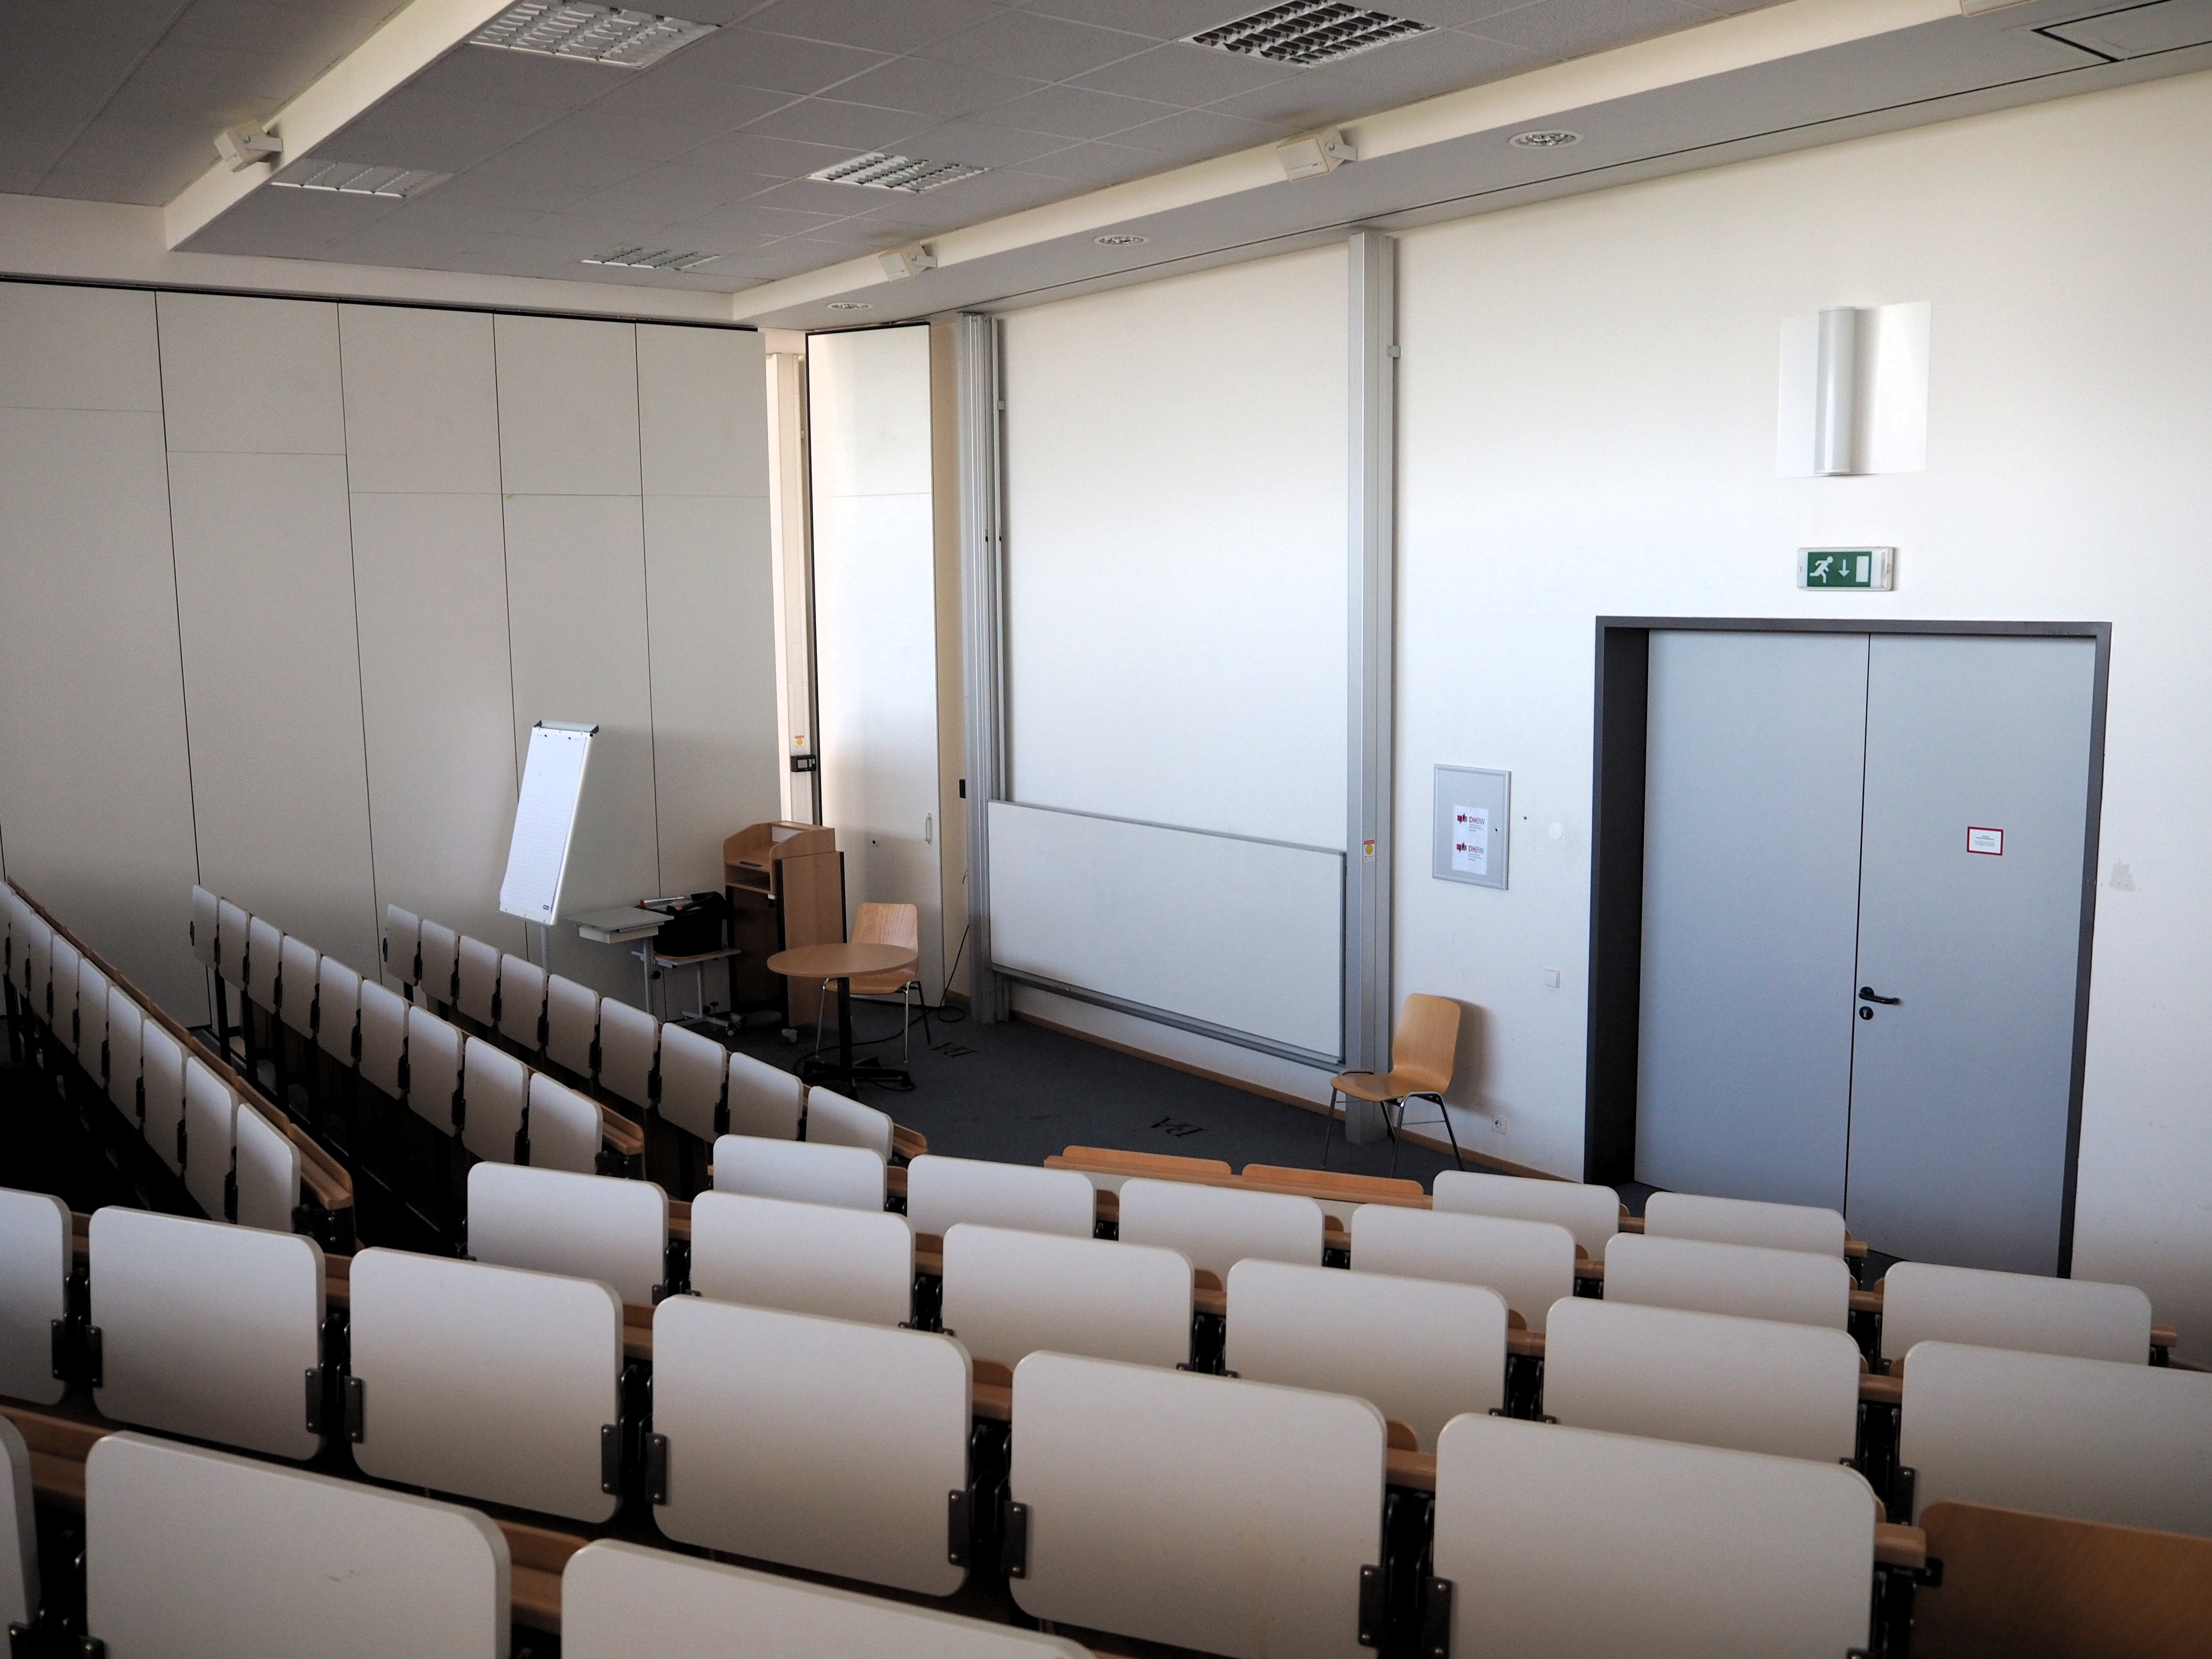
\includegraphics[width=0.25\linewidth]{images/venues/dhbw/P9280376}%
    };
    \node[inner sep=0,outer sep=0,anchor=north west] (sub-2) at (sub-1.south west) {%
      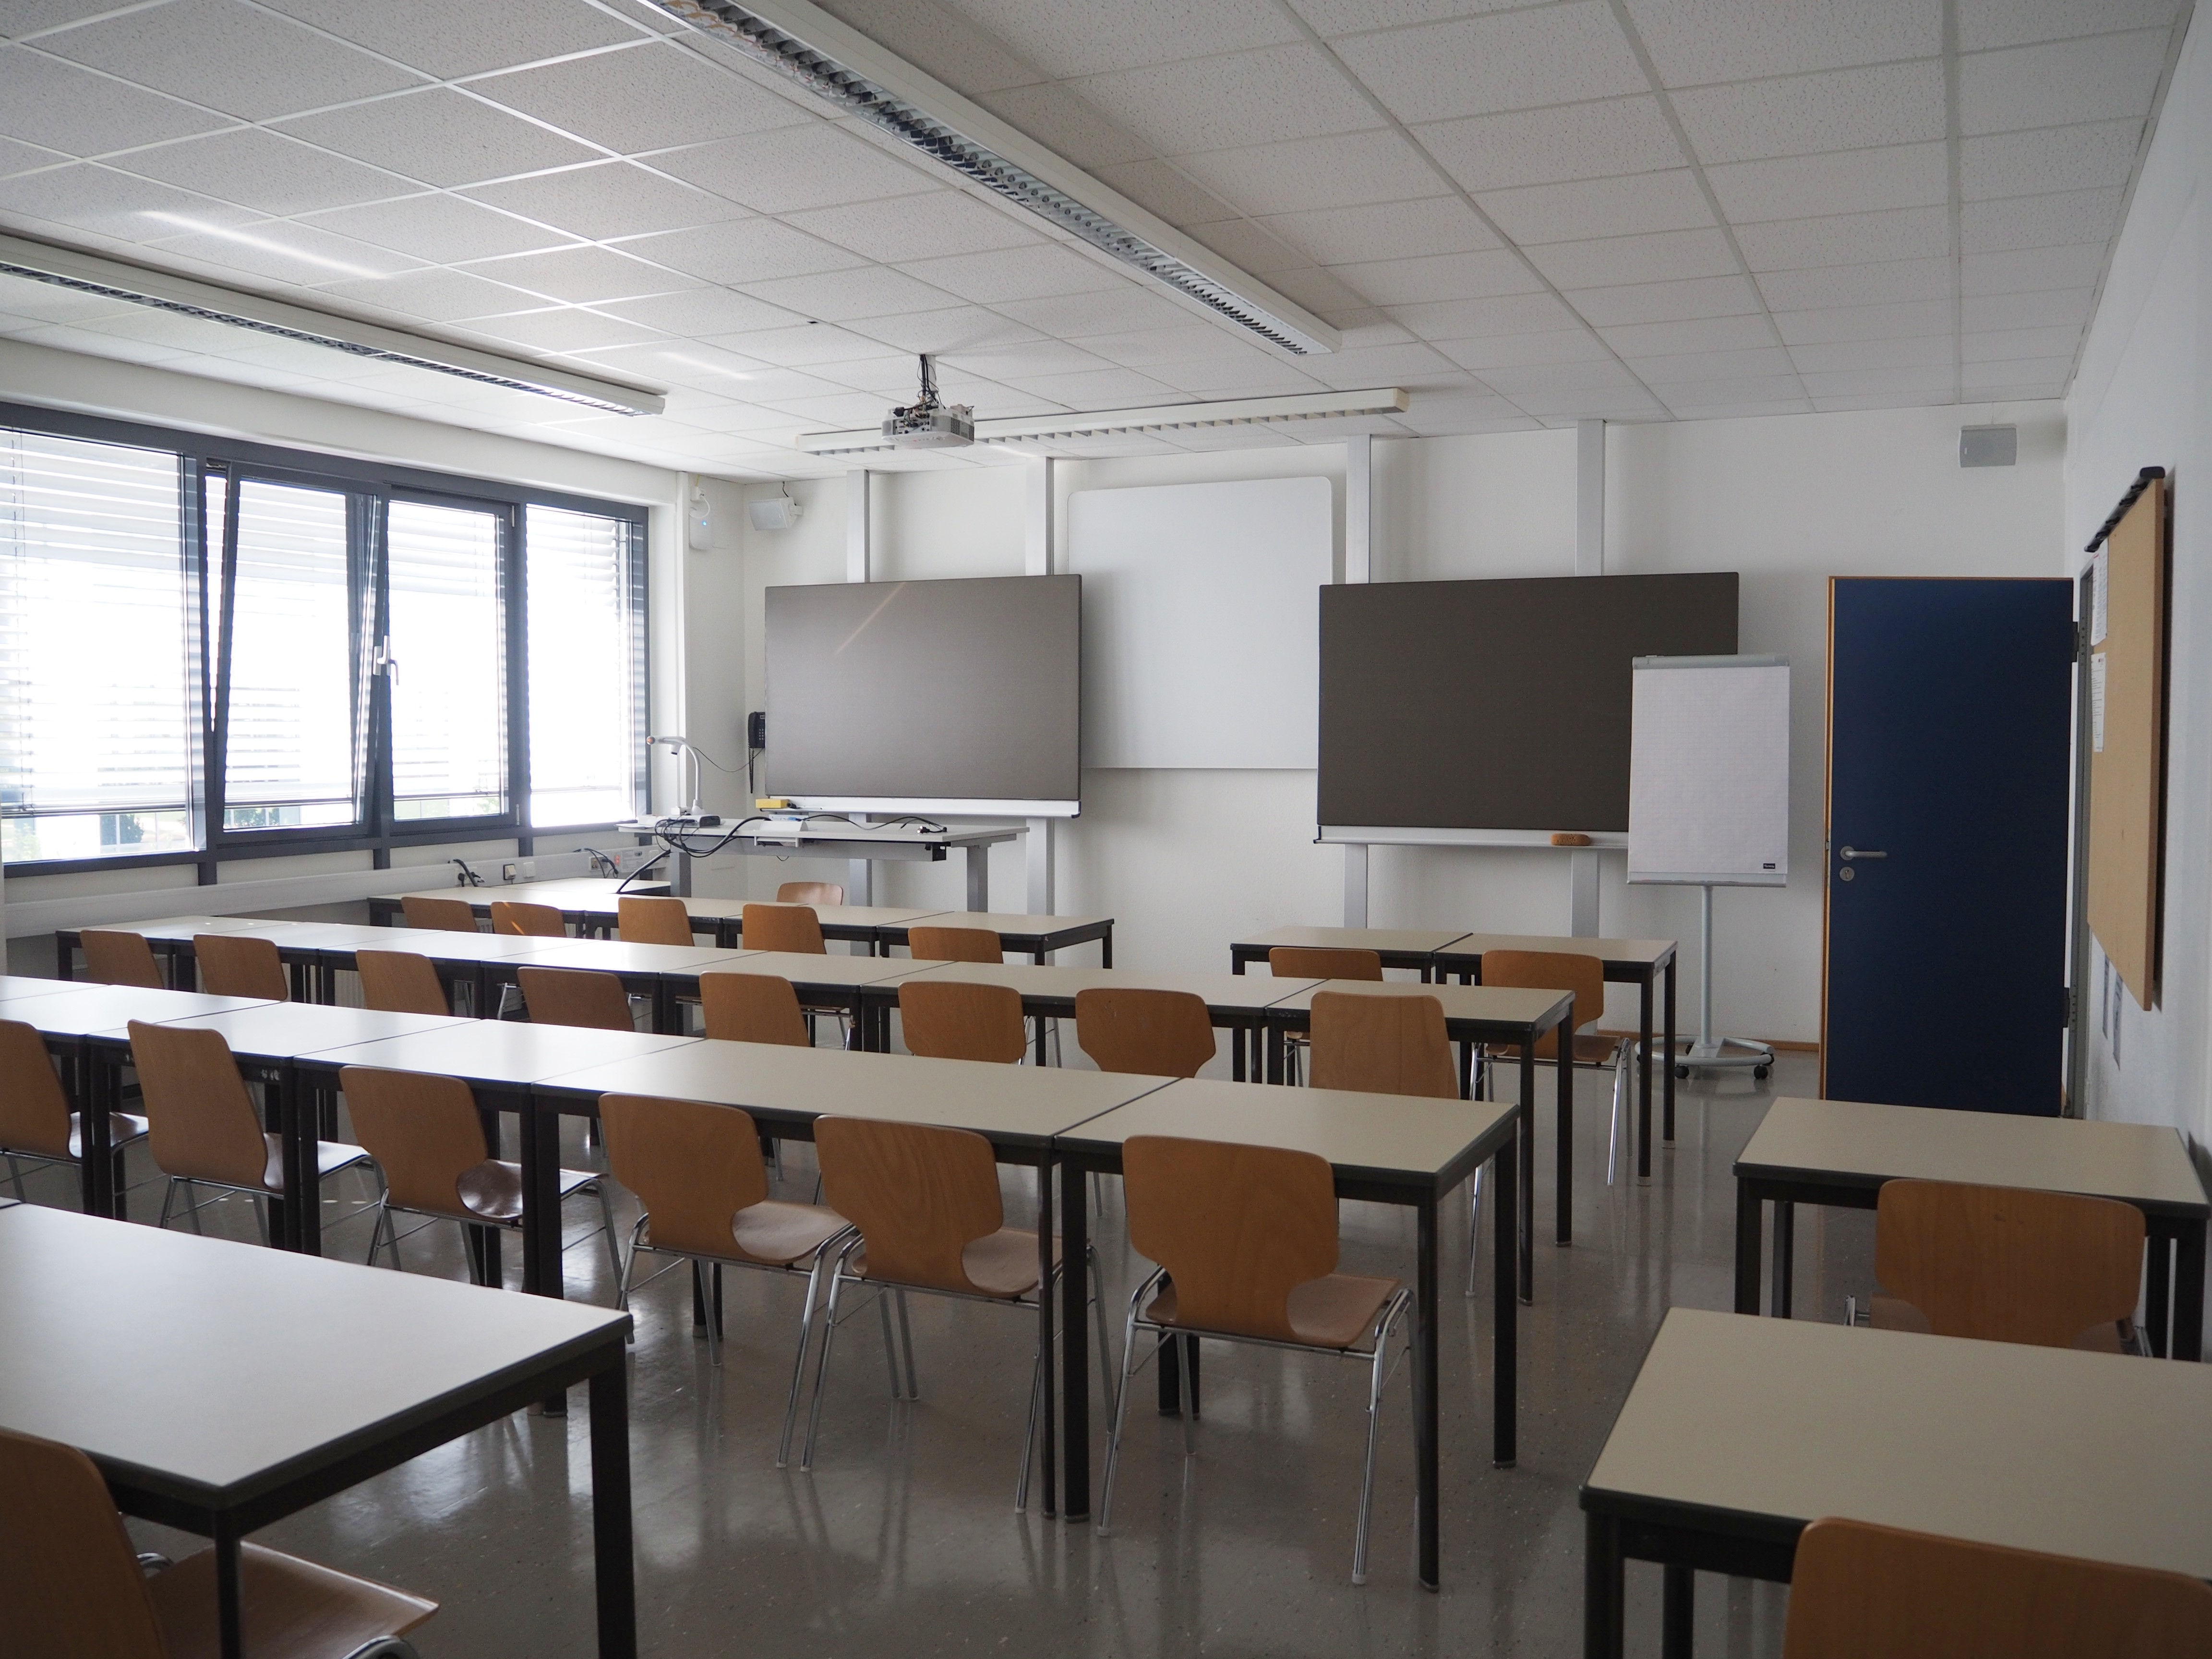
\includegraphics[width=0.25\linewidth]{images/venues/dhbw/P9280388}%
    };
    \node[inner sep=0,outer sep=0,anchor=north east] (sub-3) at (main.north west) {%
      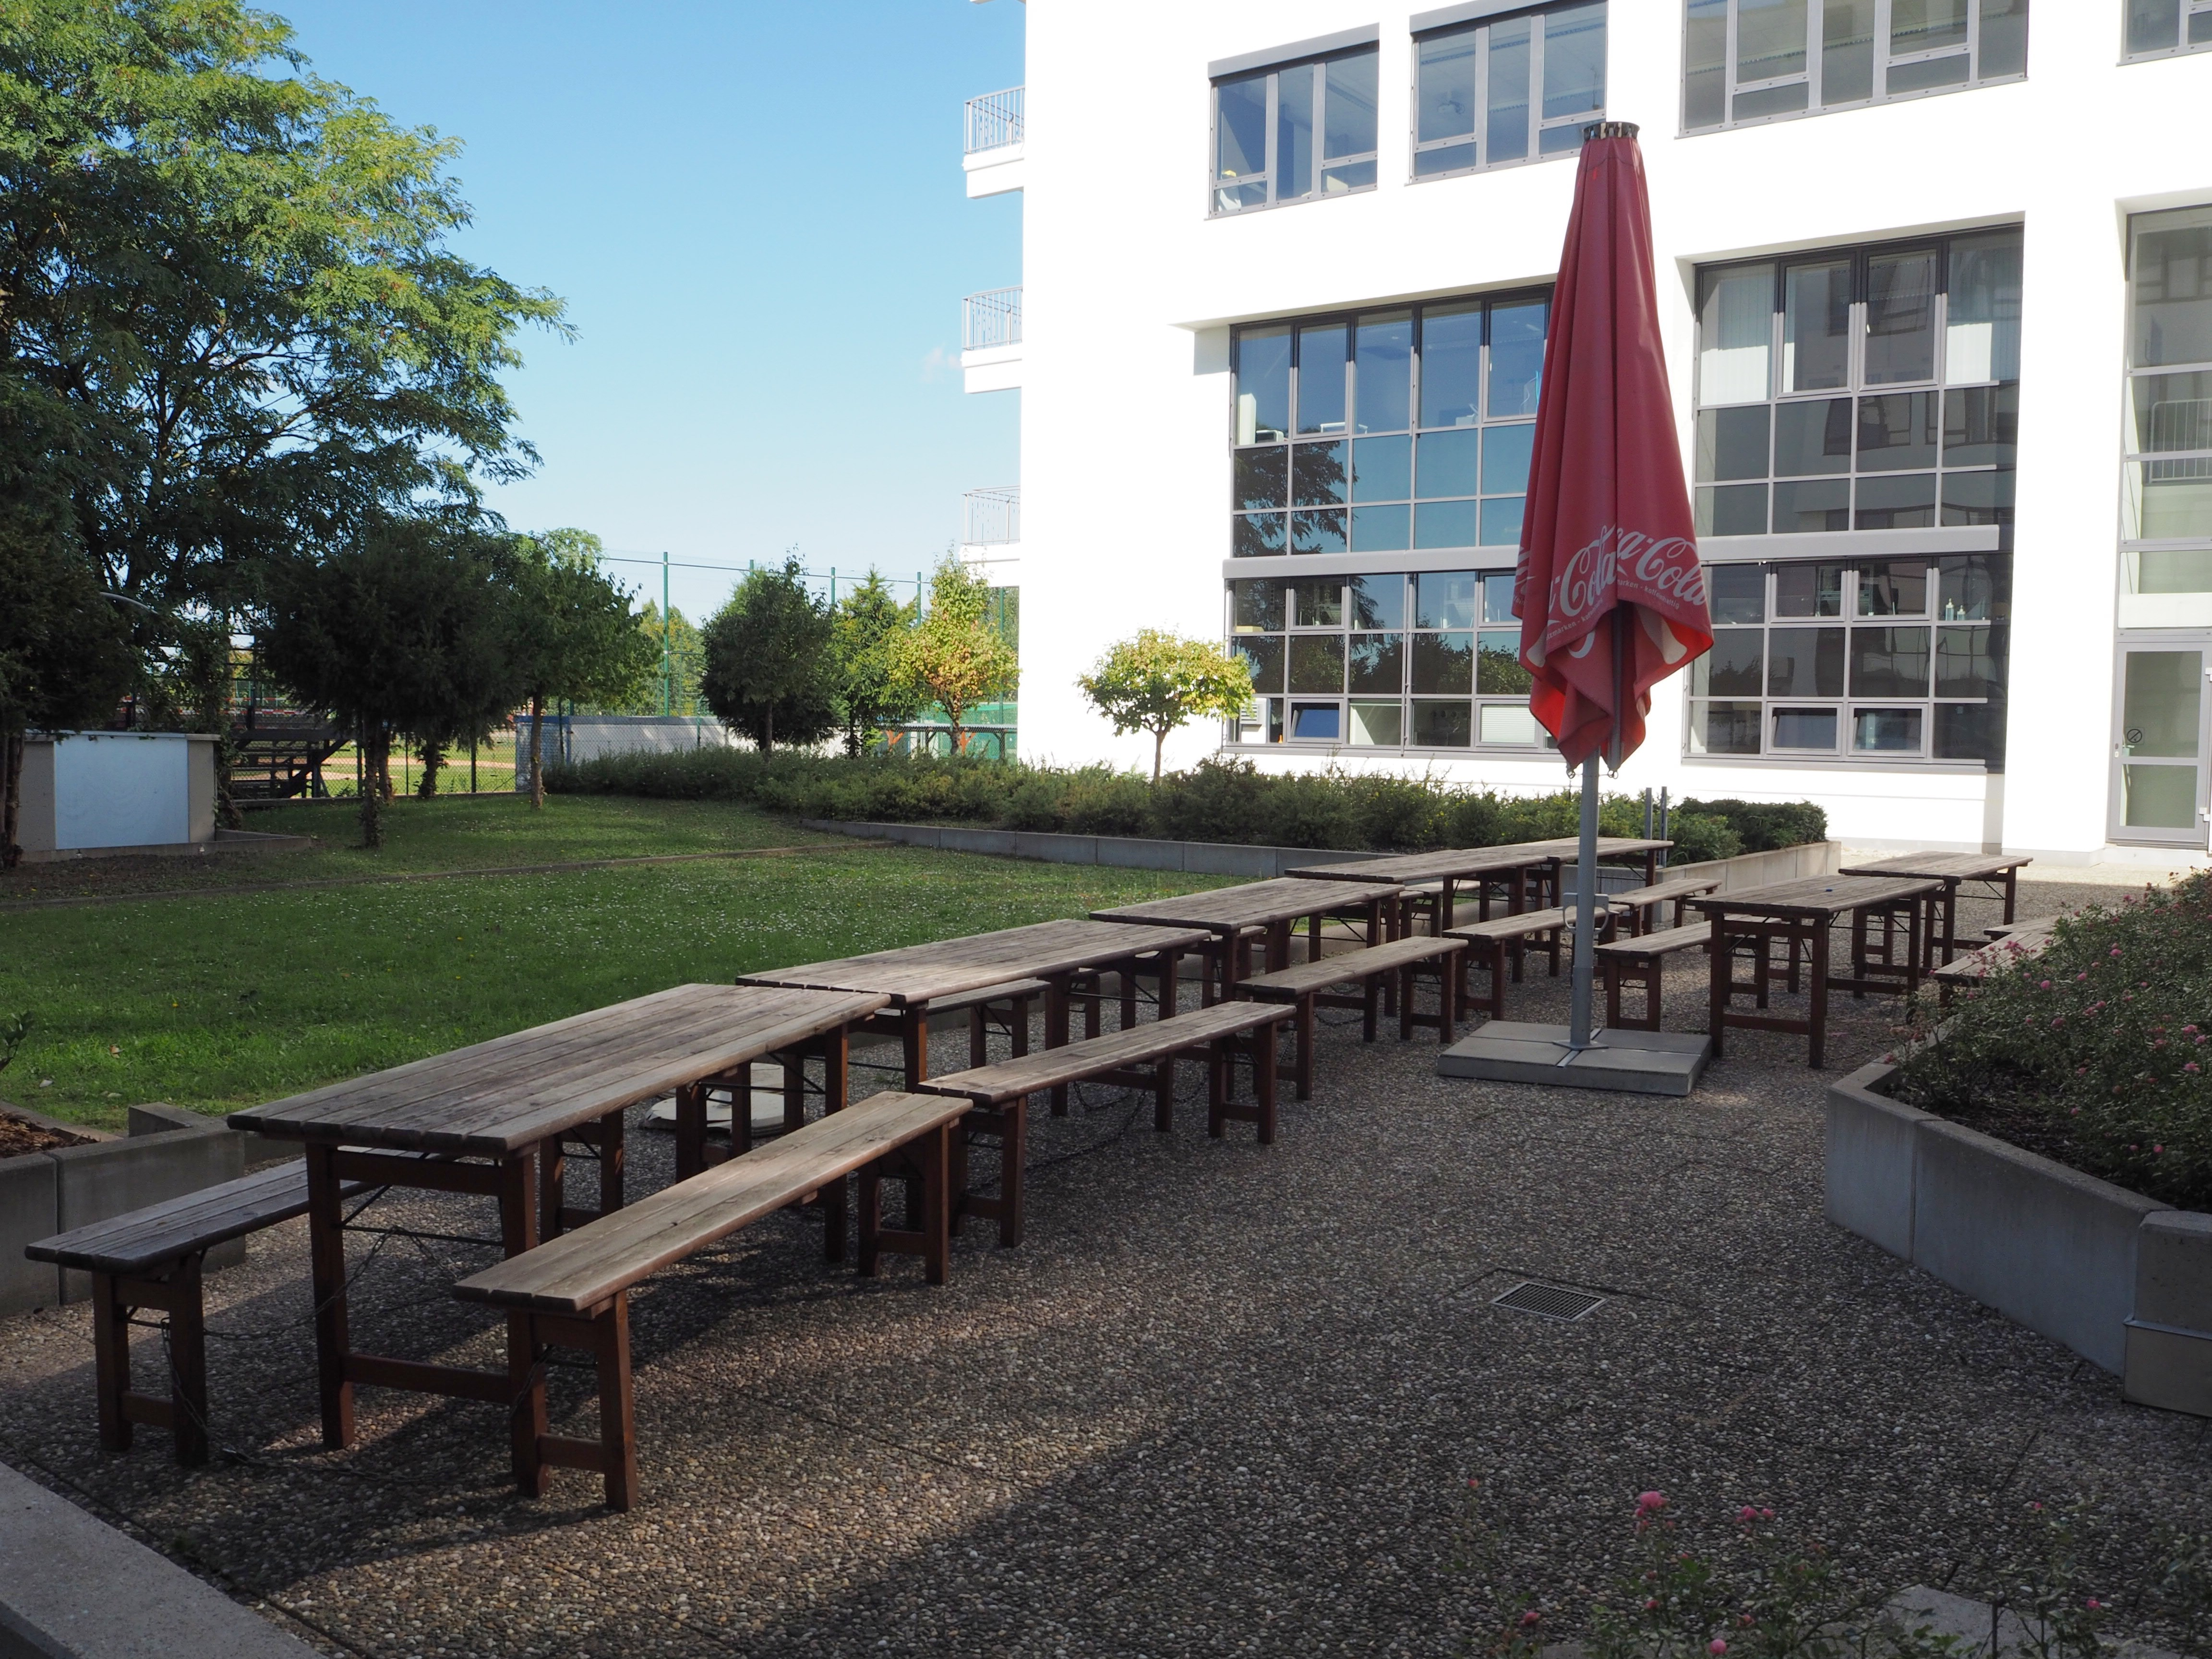
\includegraphics[width=0.25\linewidth]{images/venues/dhbw/P9280383}%
    };
    \node[inner sep=0,outer sep=0,anchor=north west] (sub-4) at (sub-3.south west) {%
      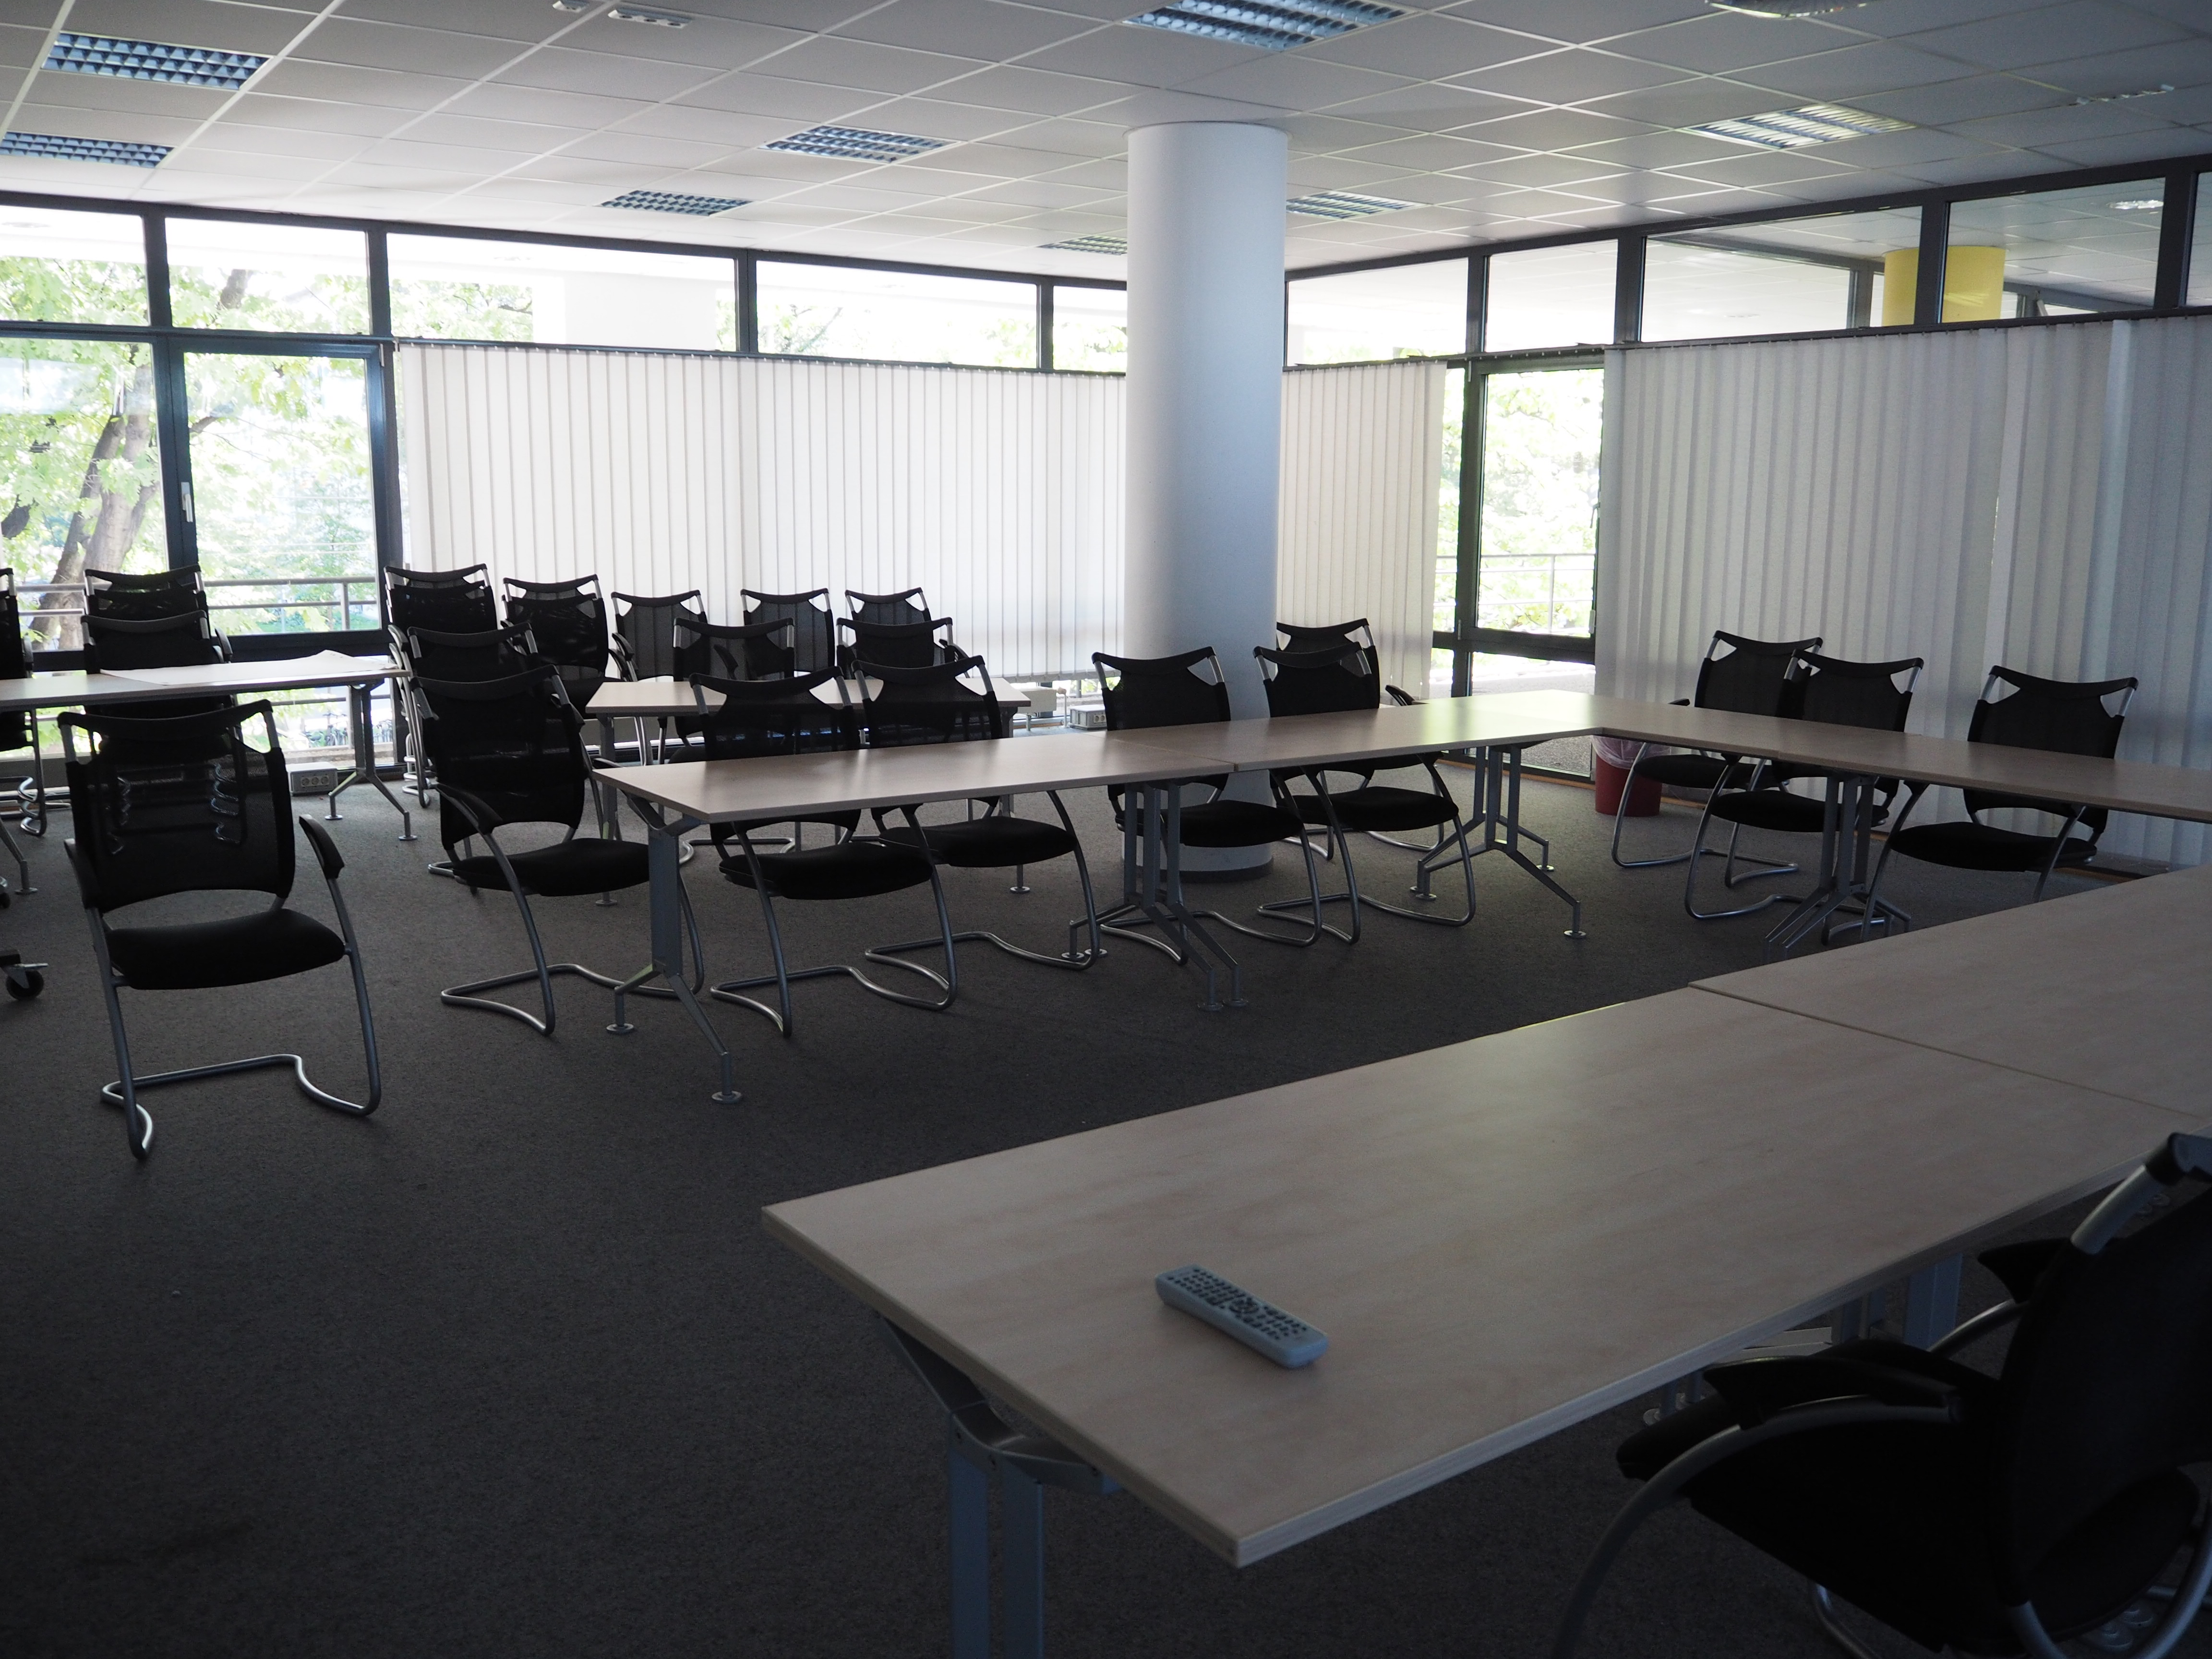
\includegraphics[width=0.25\linewidth]{images/venues/dhbw/P9280386}%
    };
  \end{scope}
  \node[anchor=south west,color=black,xshift=1ex,yshift=1ex] (label) at (sub-4.south west) {\imgtitle{Benjamin Berg}{Duale Hochschule Baden-Württemberg}{CC BY-SA 4.0}};
  \begin{scope}[on background layer]
    \node[fit=(label),inner sep=0,outer sep=0,opacity=0.6,fill=white,rounded corners] {};
  \end{scope}
\end{tikzpicture}


\begin{description}
\item[Location] off
\item[Price] gratis or cheap
\item[Rooms] audimax with 300 seats, many smaller ones
\item[Dates] end of July or later
\end{description}

The DHBW (Duale Hochschule Baden-Württemberg) offers exactly what we are looking for.
They have a large room for keynotes and some smaller rooms for talks and
also for BoFs in a single building. In addition to this the venue has
plenty of space in the lobby that we intend to transform into a lounge for
casual gatherings.

The venue is located further to the north west of the city, meaning that it is
unlikely to be within comfortable walking distance to the accommodation. However,
there is a tram station right next to the building and we are planning
to provide all attendees with tram tickets for the duration of the
conference. Furthermore if this location is chosen we are going to organize
lunch on-site as there are only limited options for lunch in the vicinity.

The venue is available from the end of July on.

\newpage

\begin{tikzpicture}[remember picture,overlay]
  \node[anchor=north west,outer sep=0,inner sep=0] (img) at (current page.north west) {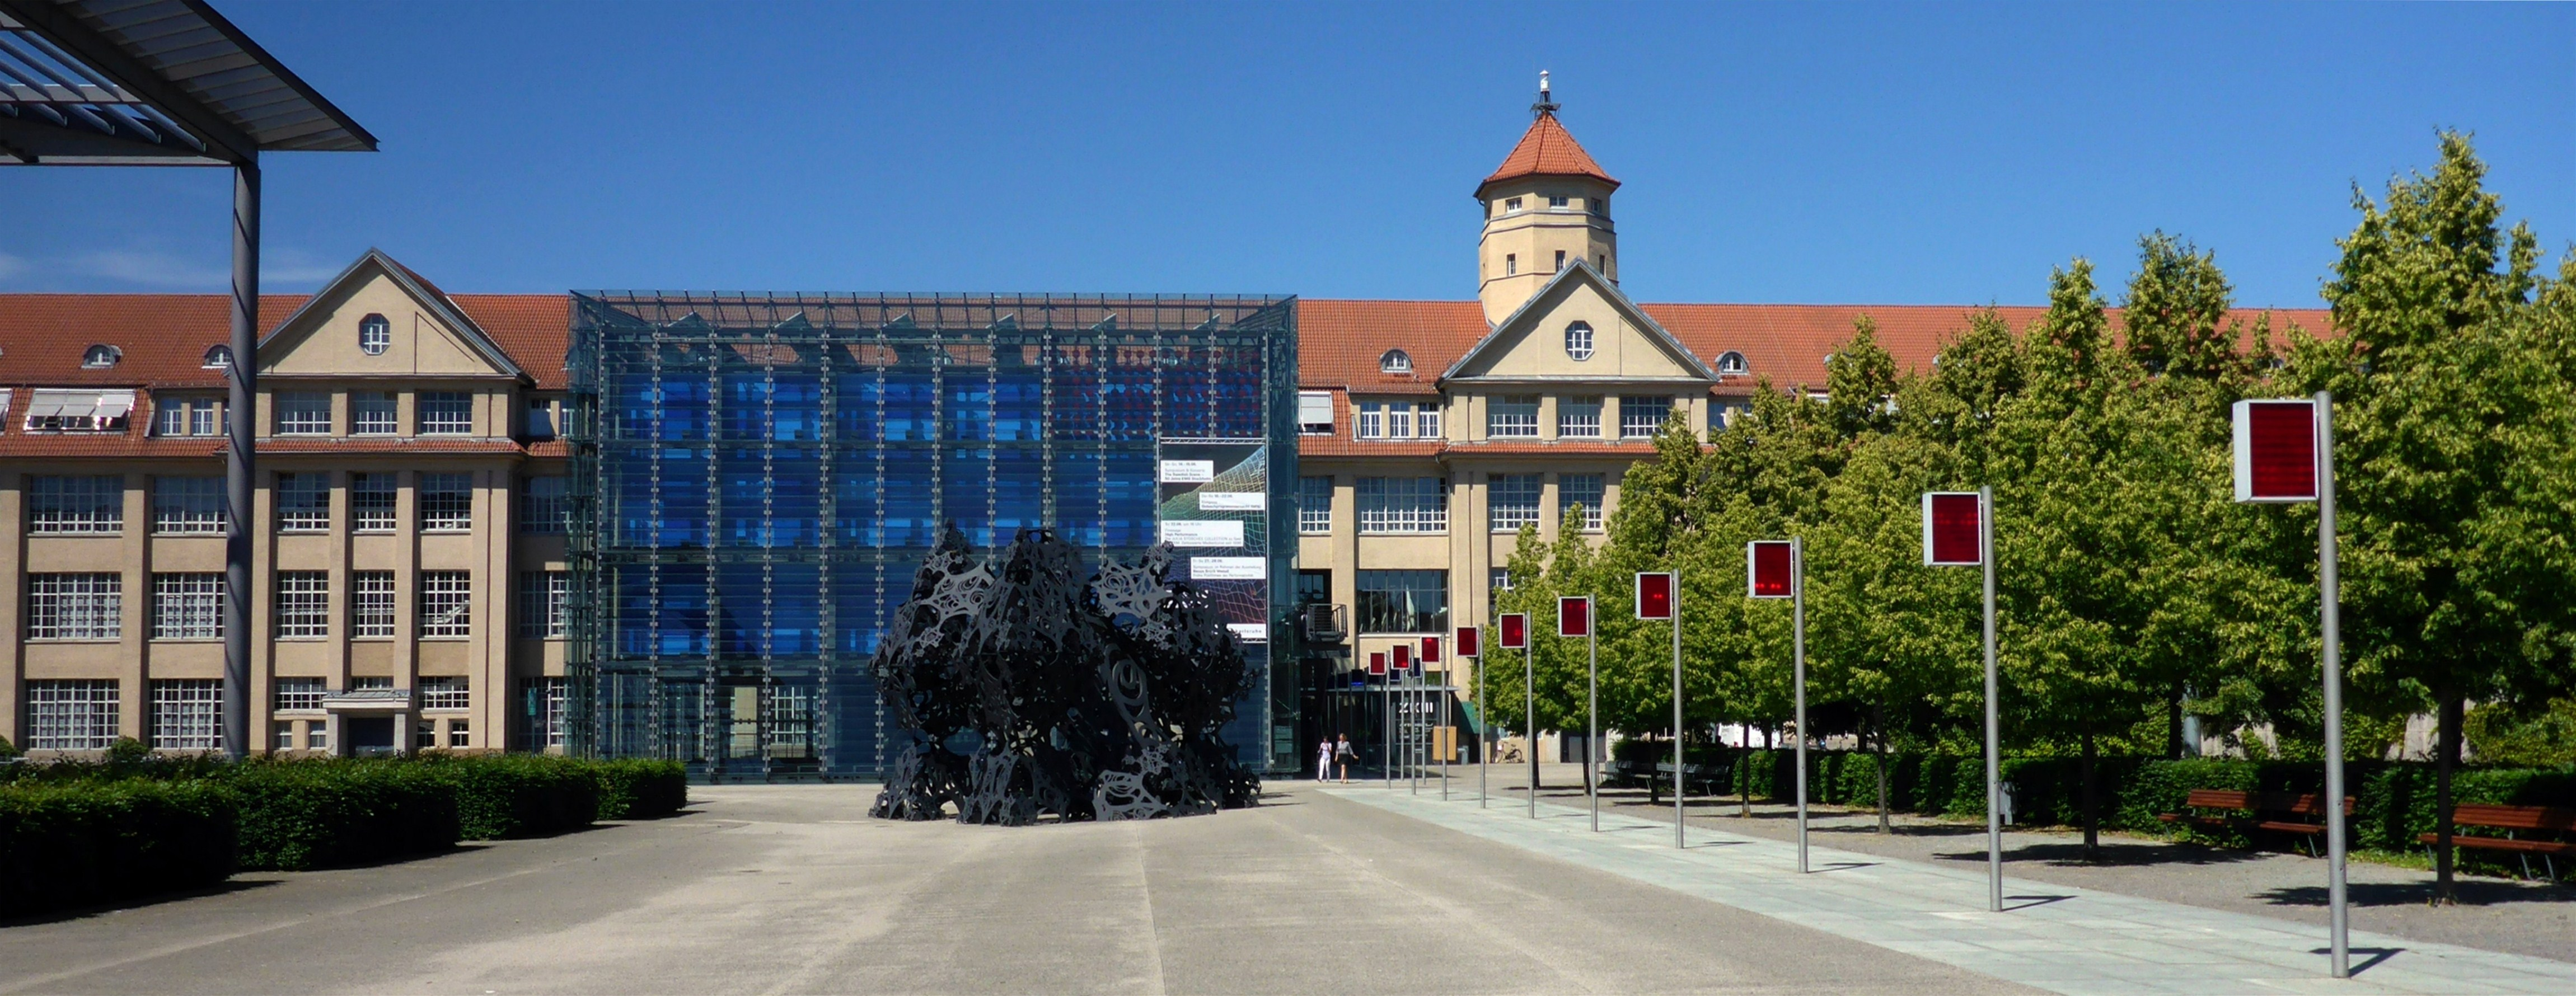
\includegraphics[width=21cm]{images/city/zkm-2.jpg}};
  \node[anchor=south west,outer sep=1ex,color=white] at (img.south west) {\imgtitle{Günter Josef Radig}{ZKM}{CC BY-NC-SA 2.0, not modified, \url{http://ka.stadtwiki.net/Datei:ZKM_2014.JPG}}};
\end{tikzpicture}

\vspace*{4.3cm}

\subsection{ZKM}
\label{zkm-venue}
\begin{description}
\item[Location] very good
\item[Price] $\sim\SI{8500}{\euro}$ for two days
\item[Rooms] one room with up to 300 seats, smaller auditorium with 100 seats
\item[Dates] 12.08.-14.08.\,2016
\end{description}

The Center for Art and Media (ZKM\footnote{Zentrum für Kunst und Medien}) is not
just a museum but a cultural institution that is unique throughout the world.
In the ZKMs own words, it is “a house for all media and genre, a house for both
spatially-based arts, such as painting, photography and sculpture as well as
time-based arts, such as film, video, media art, music, dance, theater, and performance.”

The venue has two auditoriums, the large “Medientheater” and a smaller
„Vortragsraum“. In addition to this there is a large lobby with a Café which we
would be sharing with the museum for the duration of the conference.

We would likely use this venue only for the core days, moving over to one of the
universities for the BoF sessions. As of now we have a reservation from the
12th to 14th of August.

\newpage


\begin{tikzpicture}[remember picture,overlay]
  \begin{scope}[on background layer]
    \node[anchor=north west,outer sep=0,inner sep=0] (img) at (current page.north west) {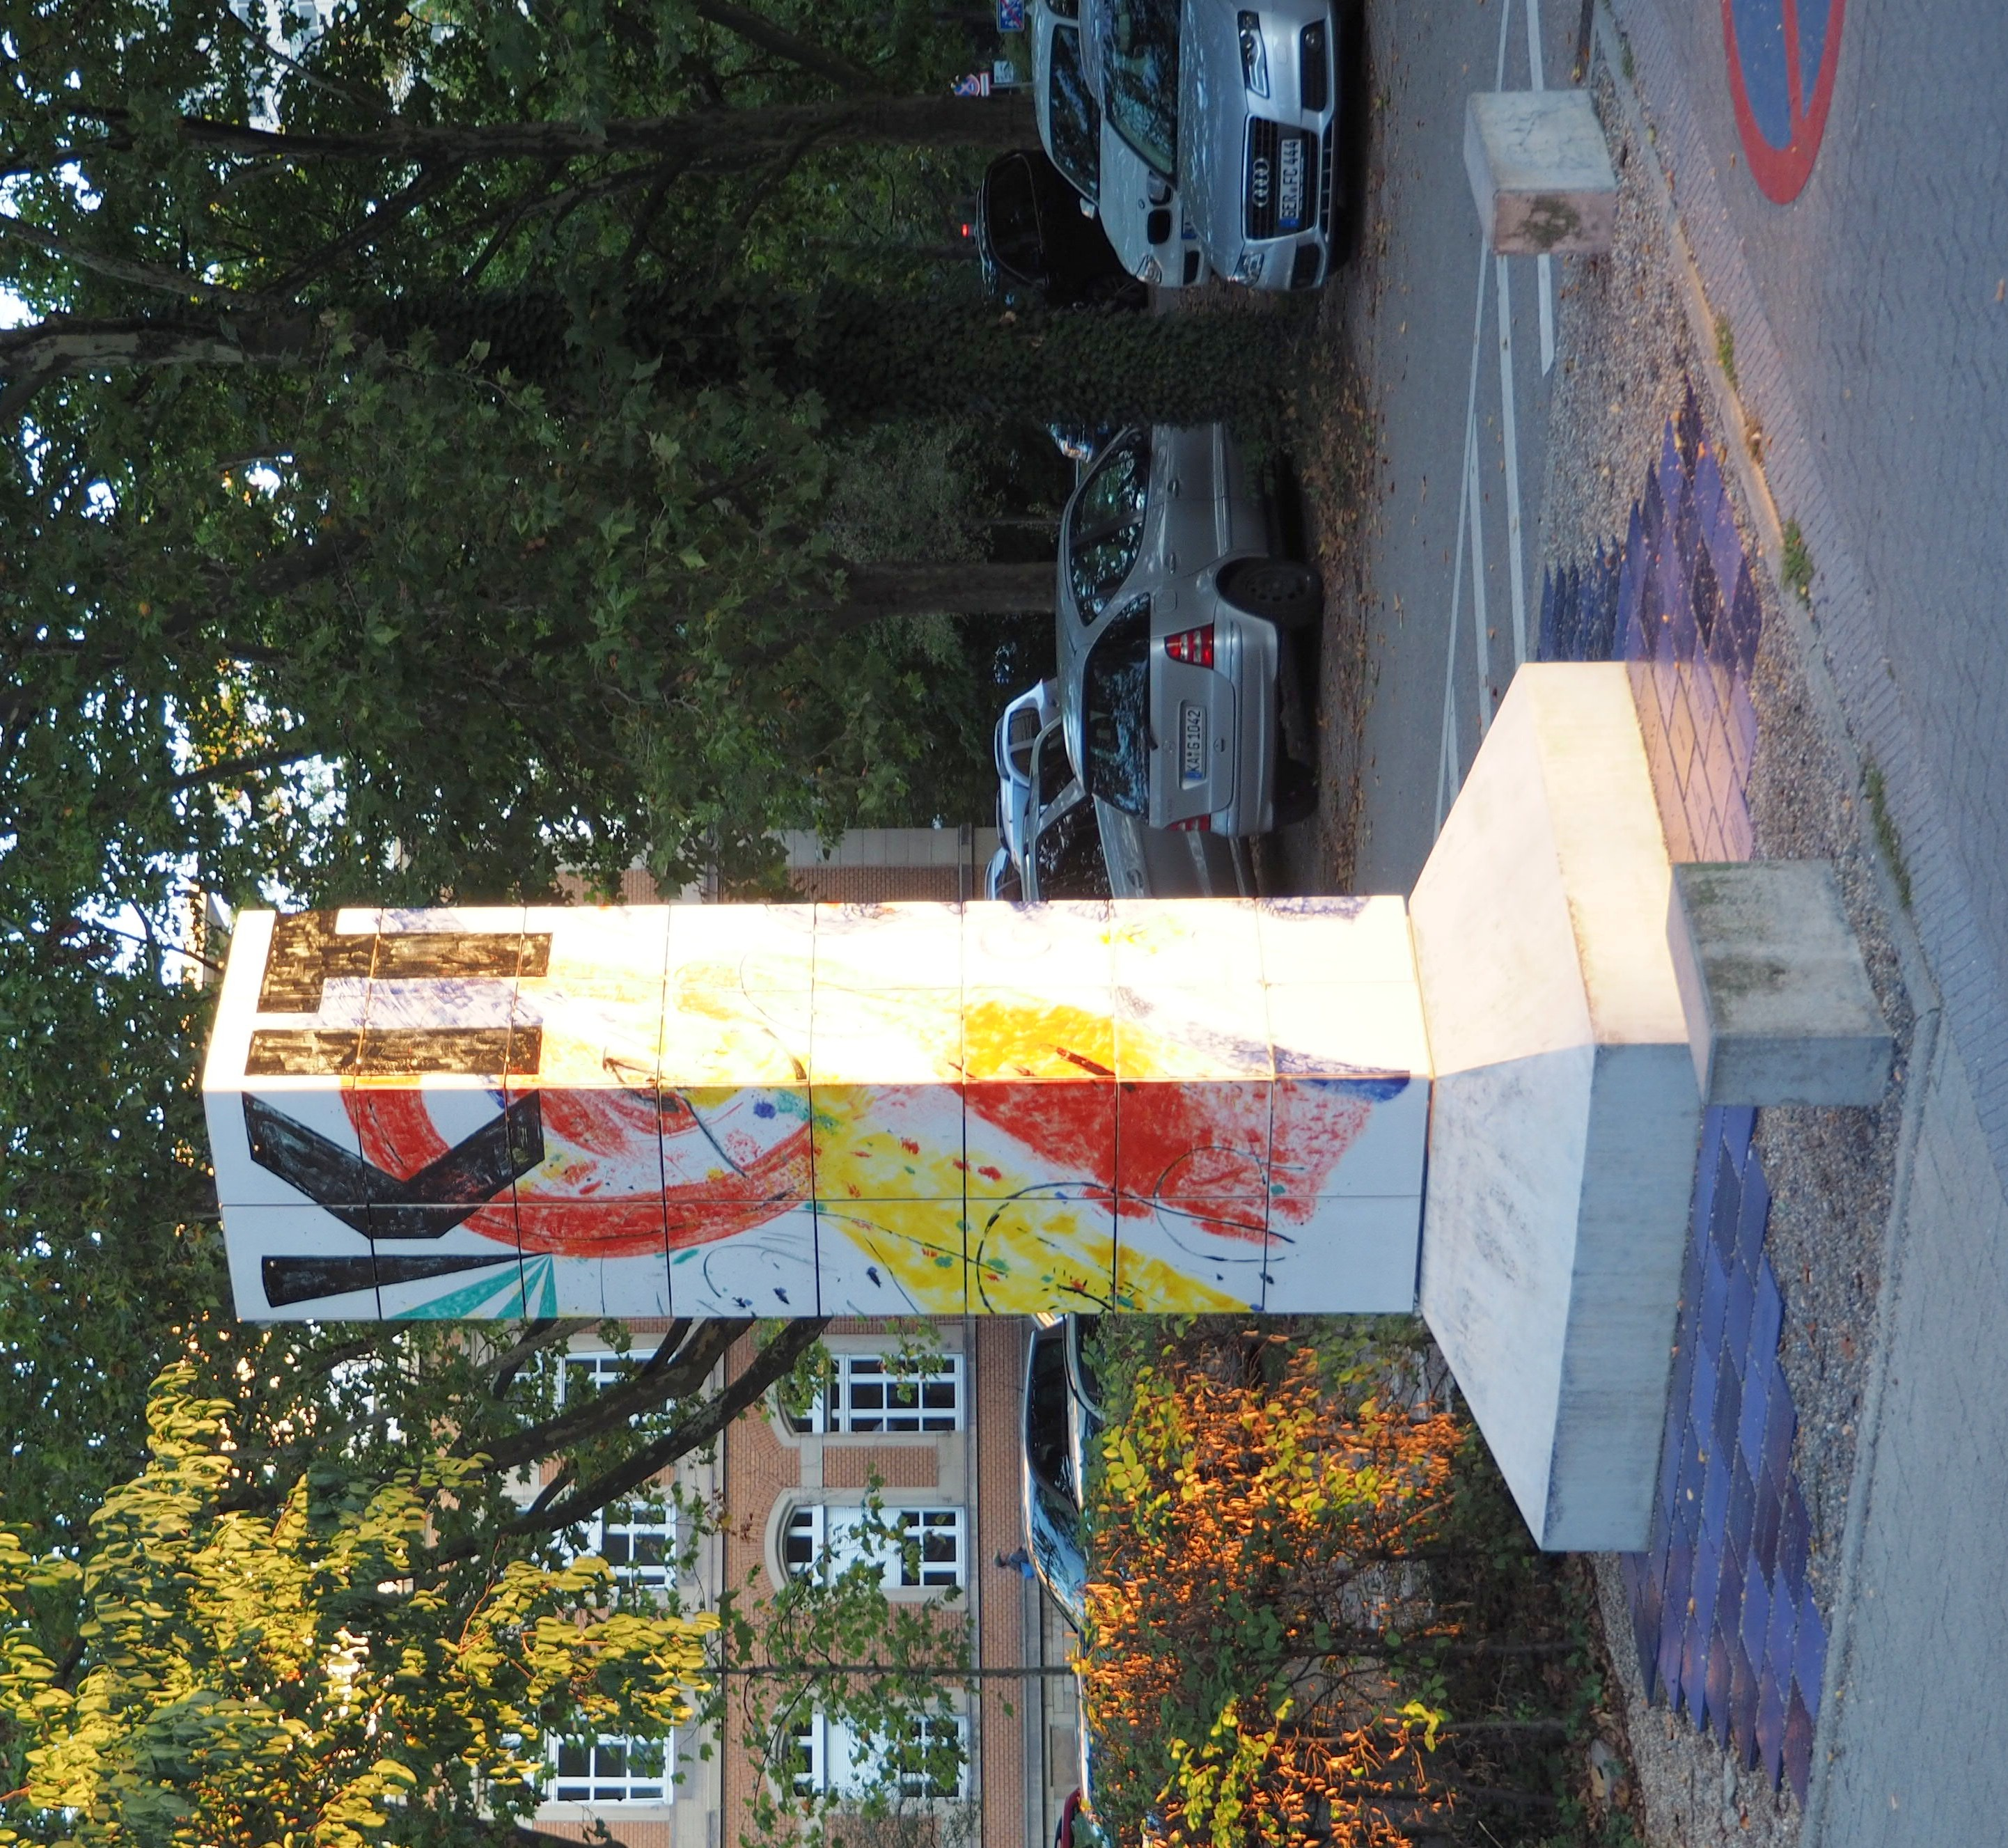
\includegraphics[width=9.5cm,angle=-90]{images/venues/kit/kit-1.jpg}};
    \node[anchor=north west,outer sep=0,inner sep=0,xshift=-1pt] (img-2) at (img.north east) {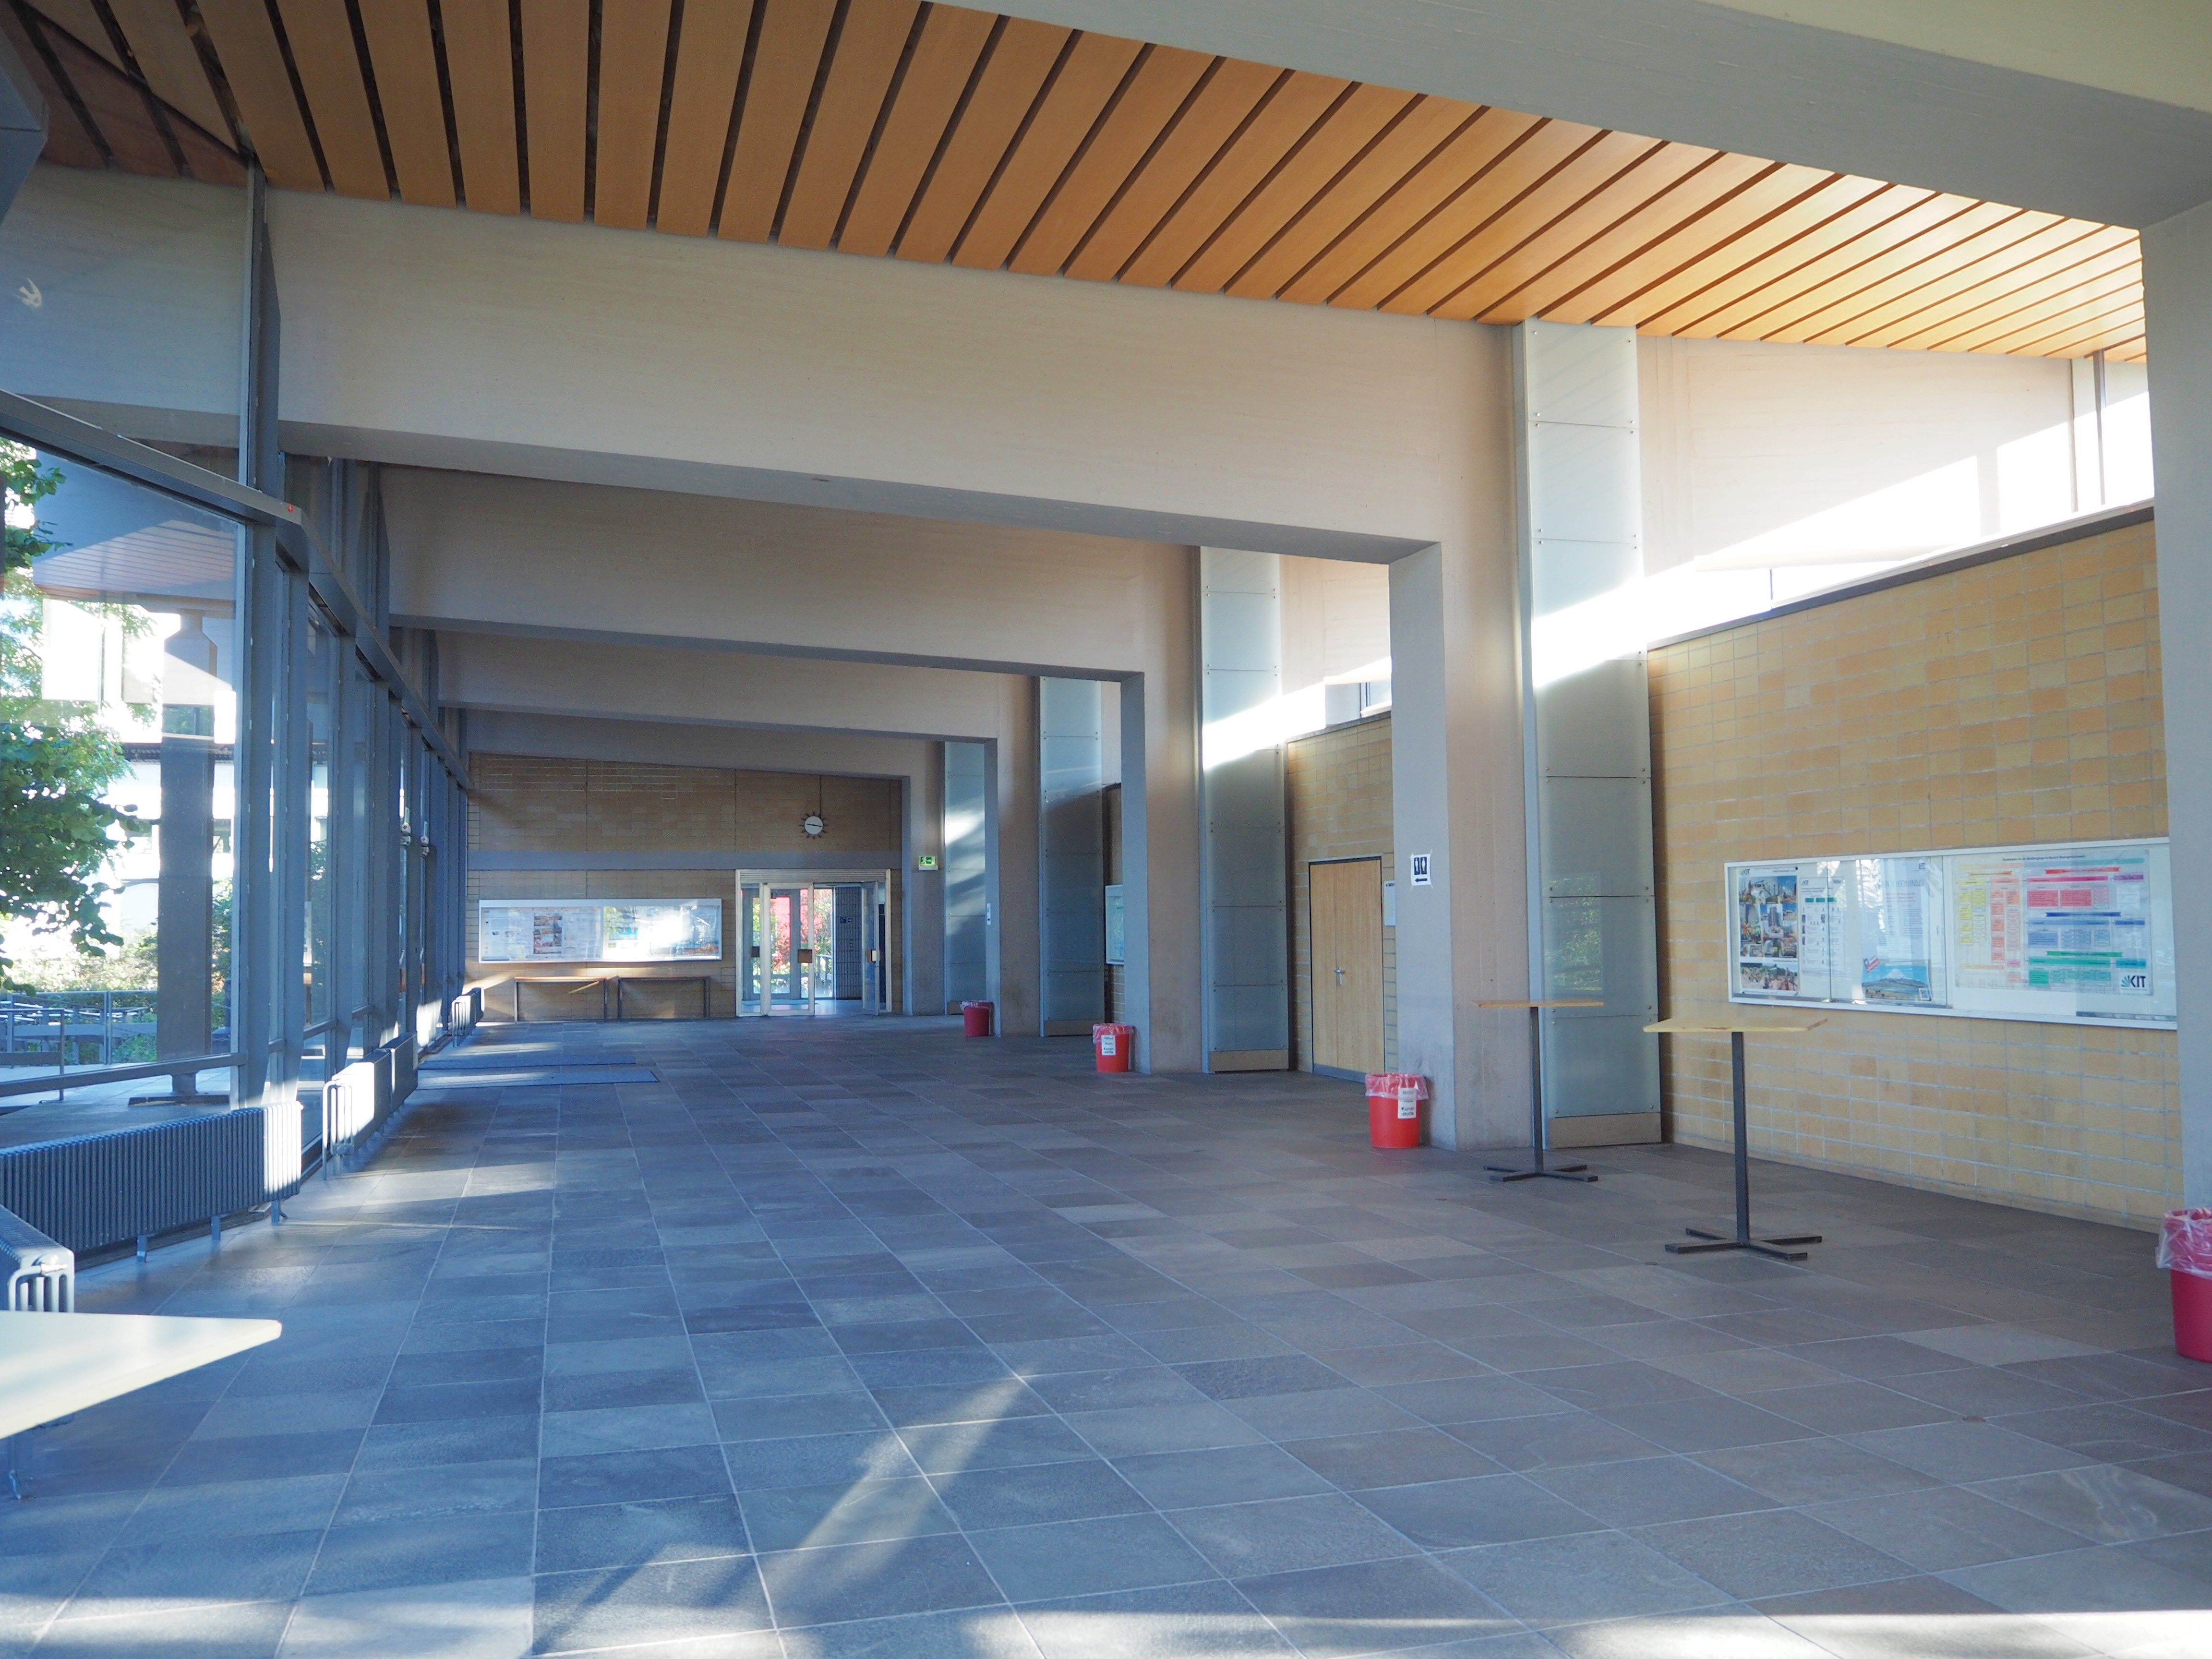
\includegraphics[height=9.5cm]{images/venues/kit/1050-1.jpg}};
  \end{scope}
  \node[anchor=south west,color=black,xshift=1ex,yshift=1ex] (label) at (img.south west) {\imgtitle{Benjamin Berg}{KIT and Building 10.50}{CC BY-SA 4.0}};
  \begin{scope}[on background layer]
    \node[fit=(label),inner sep=0,outer sep=0,opacity=0.6,fill=white,rounded corners] {};
  \end{scope}
\end{tikzpicture}

\vspace*{6cm}

\subsection{KIT South Campus (University)}%\smash{\rlap{%
%\begin{tikzpicture}
%  \pgfsetbaselinepointlater{\pgfpointanchor{baseline}{base}}
%    \node[inner sep=0,outer sep=0] at (0pt,0pt) {};
%  \begin{scope}[on background layer]
%    \node[inner sep=0,outer sep=0,anchor=north east] (main) at (\linewidth,0em) {%
%      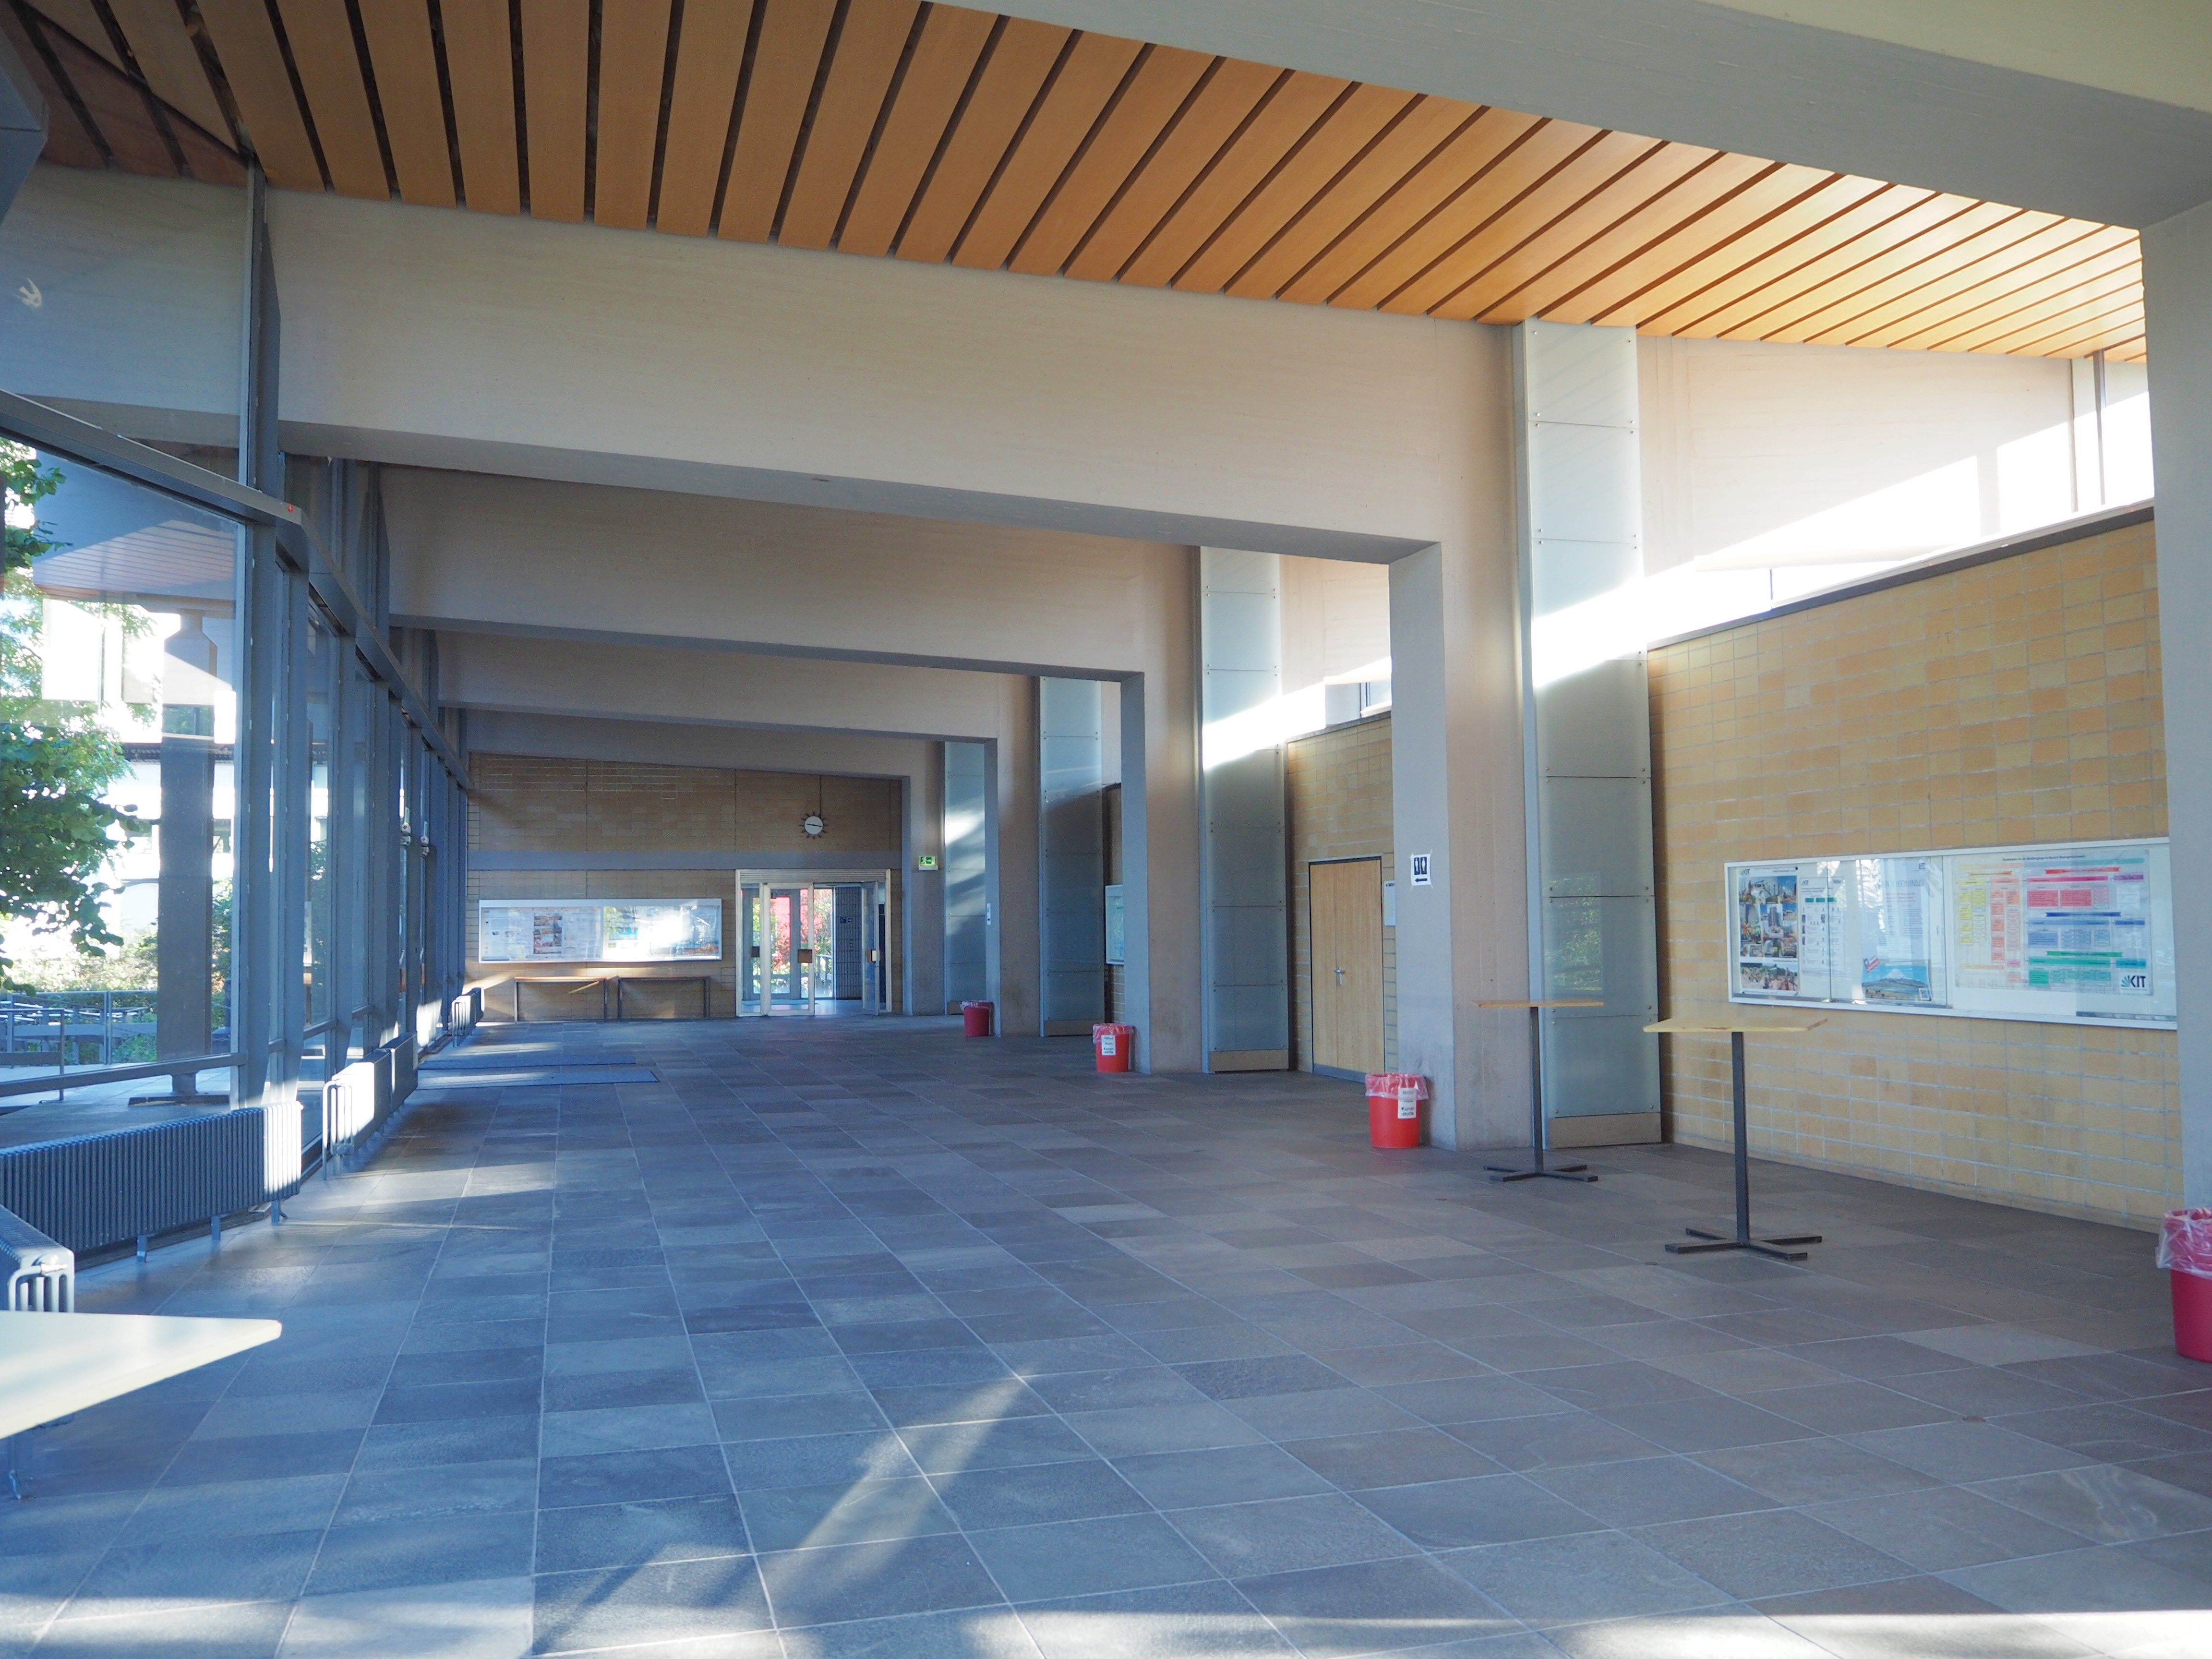
\includegraphics[width=0.4\linewidth]{images/venues/kit/1050-1.jpg}%
%    };
%    \node[coordinate] (baseline) at ($(main.north) + (0, -3em)$) {};
%  \end{scope}
%  \node[anchor=south west,color=black,xshift=1ex,yshift=1ex] (label) at (main.south west) {\rm\imgtitle{Benjamin Berg}{KIT Building 10.50}{CC BY-SA 4.0}};
%  \begin{scope}[on background layer]
%    \node[fit=(label),inner sep=0,outer sep=0,opacity=0.6,fill=white,rounded corners] {};
%  \end{scope}
%\end{tikzpicture}%
%%
%}}

\begin{description}
\item[Location] excellent
\item[Price] cheap or medium price
\item[Rooms] multiple possible locations
\item[Dates] earliest end of July, likely later
\end{description}

A third option is to hold the conference on the KIT South Campus which is
located right next to the city center. Hosting the conference on the university
campus means that all social events and the city center would be within walking
distance from the venue.

Even though the computer science department is supporting the idea of holding
GUADEC at the KIT in Karlsruhe, we were not yet able to get a confirmation from
the KIT administration. We are in contact with the administration and the
information will be forwarded as soon as possible.

\subsection{Karlshochschule}
\begin{description}
\item[Location] very good
\item[Price] unknown
\item[Rooms] unknown
\end{description}

Another venue option we are currently in contact with is the centrally
located Karlshochschule. There is to be interested to host GUADEC which
might even happen in cooperation with the ZKM. However we were not yet able
to aquire more information as there were delays due to holidays and other reasons.



\section{Concept and dates}

The traditional concept of two core days with keynotes and other 
presentation, followed by a two-day hackfest was proven to be a winning 
formula. We intend to keep those basics and add a little twist.

We plan to run a pre-event on the Friday, especially designed for 
students in computer sciences degrees from the various universities in 
Karlsruhe. The pre-event includes a general introduction to free and 
open source software and a more specific overview over the GNOME 
project and is followed by a few hands-on sessions. As two of the 
members of the organizing team are teaching at DHBW, one of the 
universities, we will be able to seamlessly integrate some particular 
aspects of the GNOME projects with topics taught at university. 
Ideally, we would like to involve our GSoC students as much as 
possible, especially during the hands-on sessions, in order to lower 
the initial barriers by creating a stimulating environment where the 
students will feel that they are working with peers.

Furthermore, we plan to host the Sunday lecture session at ZKM, where 
the end of the day can then be spent discovering the incredible variety 
of art exhibitions and challenging each other at various games.

In summary, the event will be scheduled as follows:

Friday 05.08.2016:
\begin{itemize}
\item Pre-event for students
\item Registration
\item Social event at AKK or Z10
\end{itemize}

Saturday 06.08.2016:
\begin{itemize}
\item  Core day I
\item  Social event at XXX
\end{itemize}

Sunday 07.08.2016:
\begin{itemize}
\item  Core day II at ZKM
\item  AGM
\item  GSoC Student Talks
\end{itemize}

Monday 08.08.2016:
\begin{itemize}
\item  Hackfest day I
\item  Visit of the Hoepfner Brewery
\end{itemize}

Tuesday 09.08.2016:
\begin{itemize}
\item  Hackfest day II
\item  Picnic in the “Schlossgarten”
\end{itemize}


\newpage

\section{Social Events}

An important aspect of a conference like GUADEC is to meet in a less formal
environment and make new friends in the community. We plan to host multiple
social events for everyone to attend, if at all possible we will try to
provide free drinks or even free food at some of the events.

\begin{multicols}{2}
\raggedcolumns

\subsection{AKK/Z10 Beer Event}

With the AKK and Z10 we have two non-profits run by the student community that
maintain bars close to the University (KIT South Campus).
Both of these locations are ideal as they are kept by volunteers and with just
a couple of volunteers of our own and relatively little money we can
serve drinks to all conference attendees free of charge all night long.

\subsection{Football and Games}

It is customary for GUADEC to host a football game on one of the evenings. We will
rent a football field. By working together with a student organization at the
KIT we can rent one on the university campus free of charge.

\subsection{Picnic}

Karlsruhe has a nice park to the north of the castle which provides a beautiful
place to play games and enjoy the day. One one evening we would like to do
a picnic in this park.

\columnbreak

\begin{tikzpicture}
  \node[outer sep=0,inner sep=0] (img) {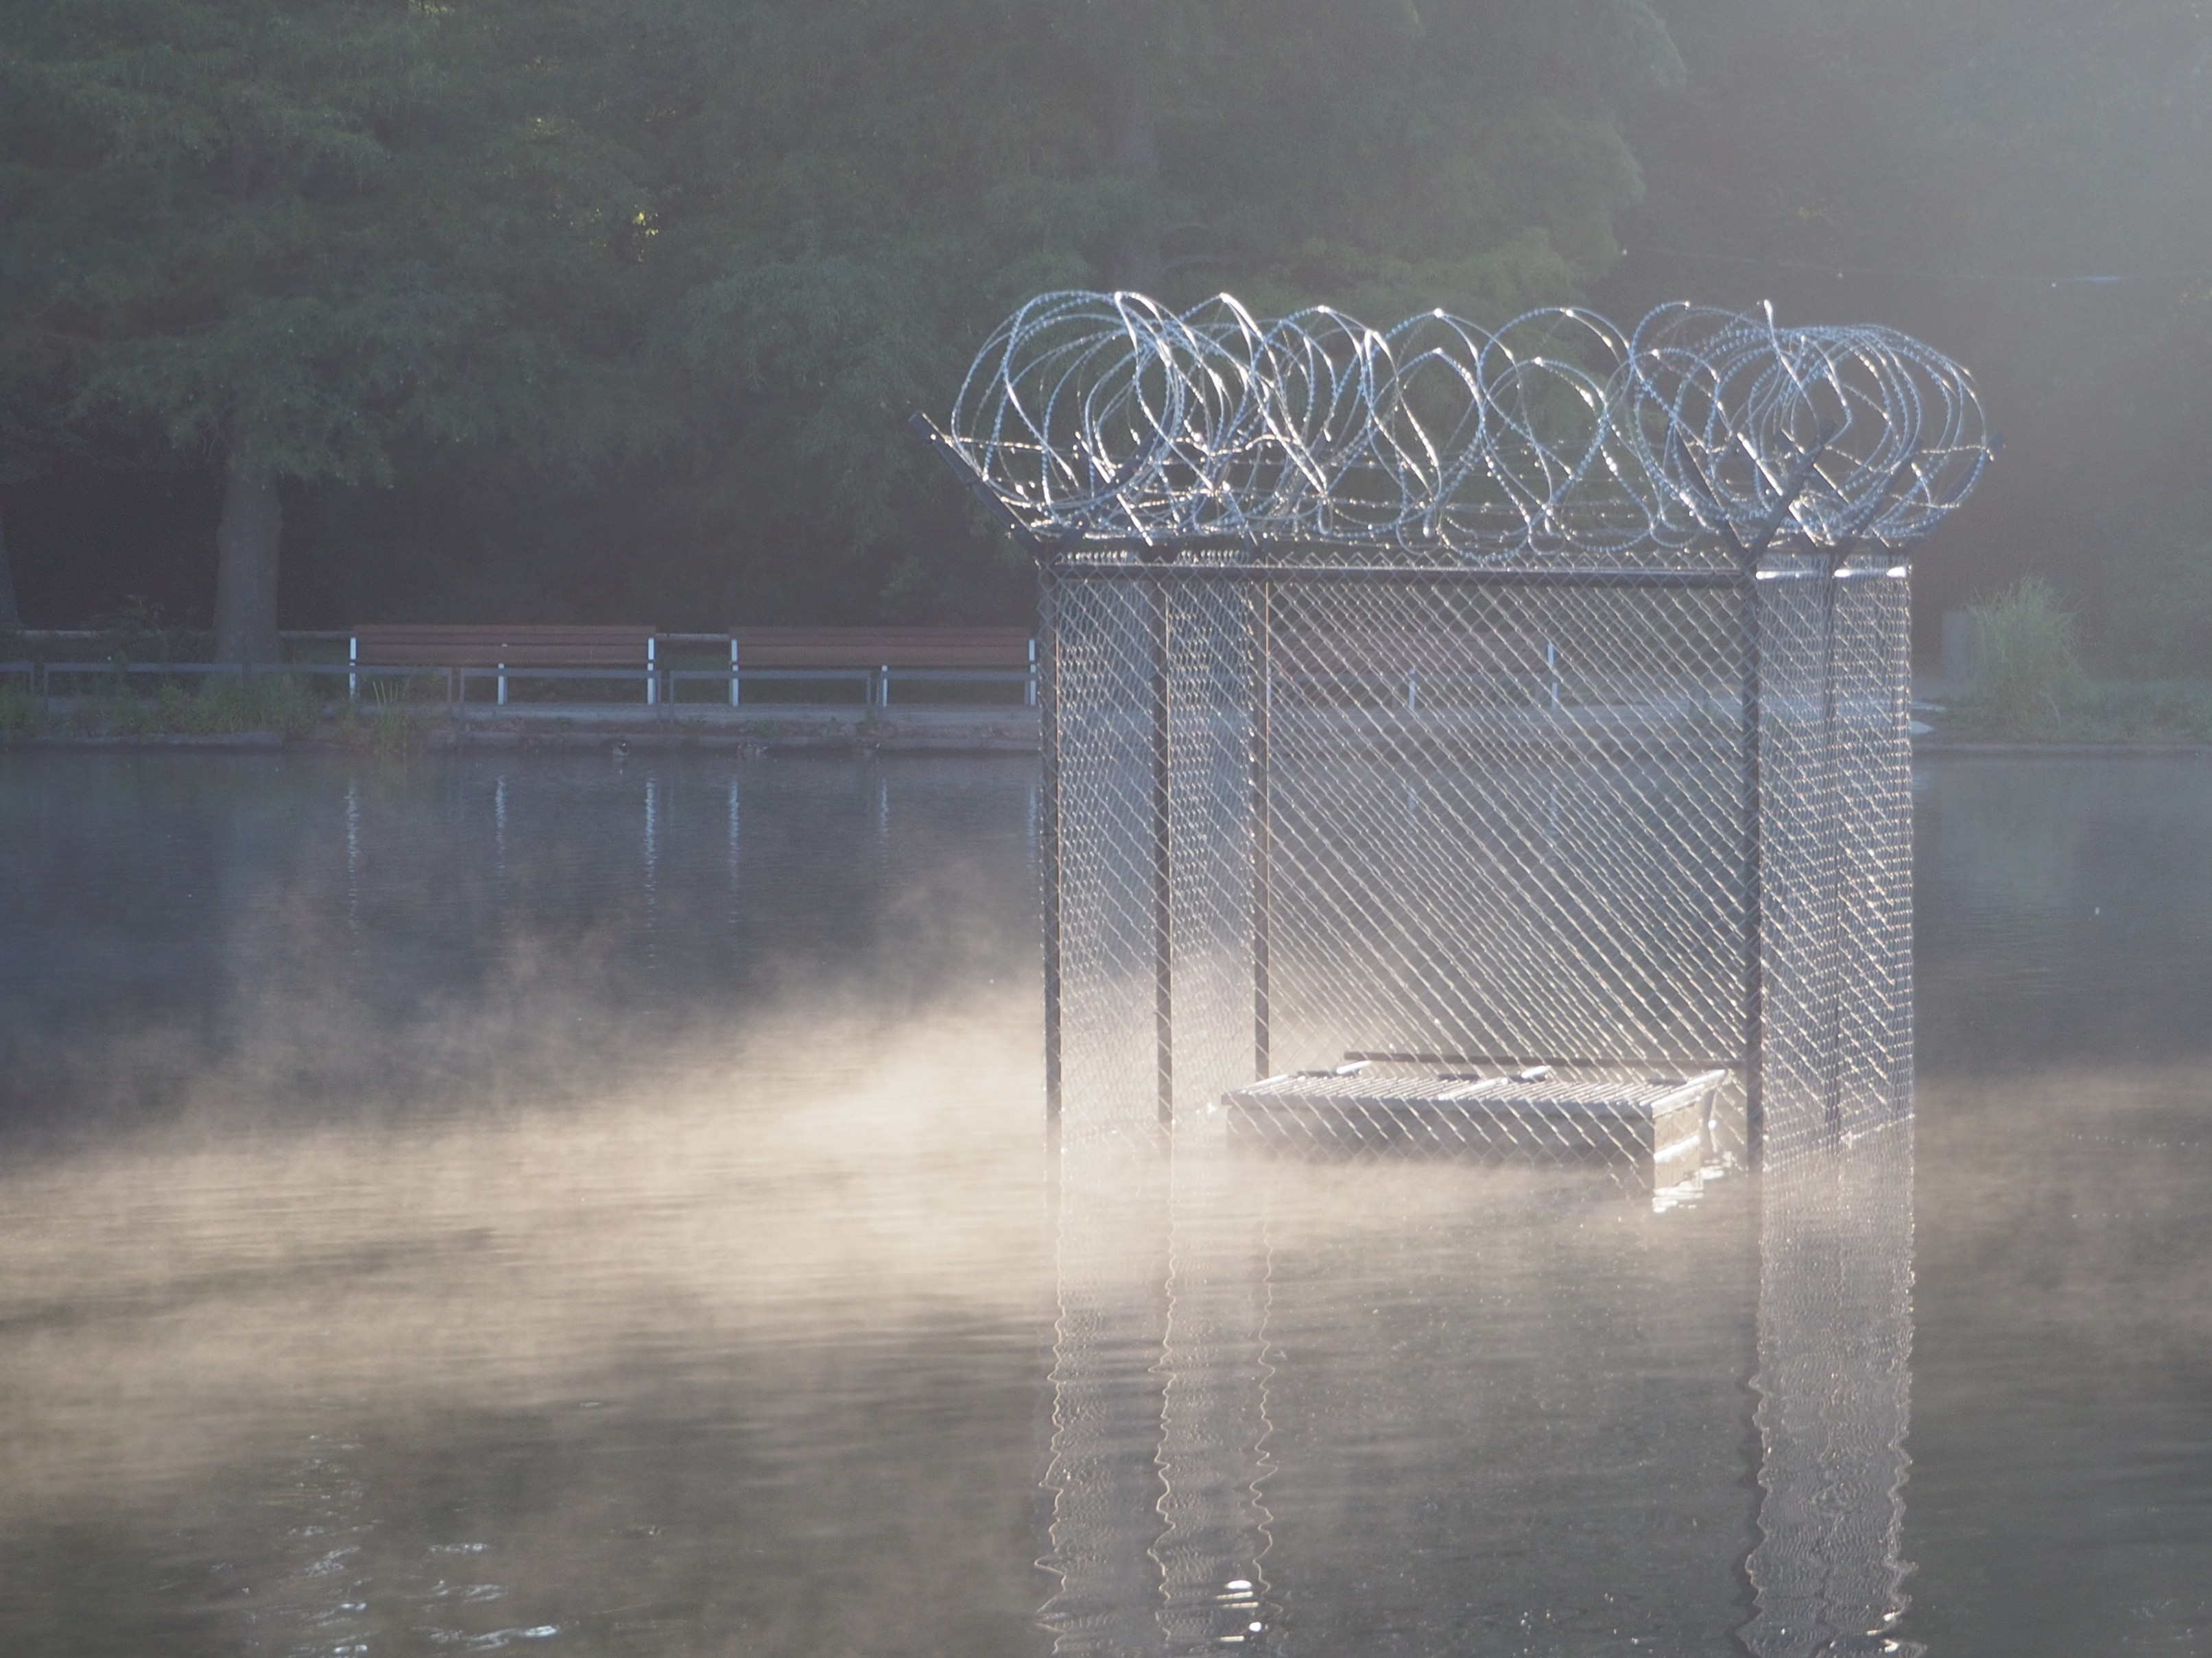
\includegraphics[width=\linewidth]{images/city/art-1.jpg}};
  \node[anchor=south west,color=white,outer sep=1ex] at (img.south west) {\imgtitle{Photo by Benjamin Berg}{Art installation, ZKM}{CC BY-SA 4.0}{}};
\end{tikzpicture}

\subsection{Center for Art and Media (ZKM)}

XXX probably makes sense to list it here, if we claim that we will organize
a tour of the ZKM. Lorem ipsum dolor sit amet, consectetur adipiscing elit, sed do eiusmod tempor incididunt ut labore et dolore magna aliqua. Ut enim ad minim veniam, quis nostrud exercitation ullamco laboris nisi ut aliquip ex ea commodo consequat.

\subsection{Barbecue}

On the first evening we are planning to barbecue. We can provide attendees with
food and drinks throughout the evening as they are arriving in Karlsruhe.



\end{multicols}

\newpage

\section{Travel}

\subsection{Airports and connections}

\subsubsection{Frankfurt International Airport}

According to wikipedia there are "107 airlines flying to 275 destinations in 111 countries from Frankfurt Airport, with approximately 1,365 flights per day". Frankfurt is one of the major long-haul hubs of Europe. Karlsruhe, only a stone-throw away is hence accessible from all around the world.

\url{http://www.frankfurt-airport.de}

From Frankfurt Airport, Karlsruhe can be reached by train or by bus. While the shortest, but also most expensive option is by train (ICE 1h05, 40 Euro), bus trips take about 2h00 (from 1h45 to 3h00) for about a fourth of the price.

We recommend \url{https://www.busliniensuche.de} to find the best option.

\iffalse
\subsubsection{Frankfurt Hahn}

Various airlines are connecting Frankfurt Hahn to about 30 destinations in Europe. Most of these airlines offer fairly cheap fares (Ryanair, Easyjet etc.). The airport is only accessible from Karlsruhe by bus over Mannheim or Frankfurt. The trip takes about 4 hours and costs roughly 25 euros.

\url{https://www.hahn-airport.de}
\fi

\subsubsection{Stuttgart Airport}

About 55 airlines are flying to over a 100 destinations from Stuttgart airport. The trip from Stuttgart Airport to Karlsruhe by train takes 1h35 and costs 25.50 euros. Postbus, as well as other bus lines, have offers as cheap as 5 euros. Bus trips, leaving directly at the airport, take about an hour. 

\url{http://www.flughafen-stuttgart.de}

\subsubsection{Karlsruhe Airport/Baden-Baden}

Airlines are flying to about 60 destinations around the world during summer times. The Hahn-Express, the same bus line connecting Karlsruhe to Frankfurt Hahn, allows airport access within half an hour.
 
\url{https://www.baden-airpark.de}

\subsubsection{Strasbourg}

As already known per the GUADEC in 2014.
Karlsruhe can be reached via TGV or local train in about an hour.


\subsection{Bus}

Karlsruhe has a big bus terminal with direct connections to other German cities, to France, Norway, Sweden, Belgium, The UK, The Netherland, Czech Republic etc.

We recommend \url{https://www.busliniensuche.de} to find the best option.

\subsection{Train}

Karlsruhe has obviously a train station with direct connections to other German cities, to France, Norway, Sweden, Belgium, The UK, The Netherland, Czech Republic etc.

We recommend \url{https://www.db.de} to find the best option.

A team member of the organizing committee is an expert in finding the best and cheapest travel option and will be delighted to assist you in finding your way to Karlsruhe for GUADEC 2016!

\subsection{Car and Parking}

If you want to park your car in the inner city of Karlsruhe, a special ticket for 5 euros is required. 

Details can be found at:
\url{http://www.karlsruhe.de/b3/natur_und_umwelt/umweltschutz/luftreinhaltung/umweltzonen.de}

If you need assistance, the organizing committee will assist you.

\subsection{Local public transport}



The local public transport system (KVV) is a tight network of buses and trams connecting not only the different part within the city, but anchoring the city in the wider context of Baden-Würthemberg. The organizing committee is committed to investigate the possibility to get special day passes for all participants for the duration of the event. Alternatively there are day passes for 5 people for 9euros.

Karlsruhe is a compact city. The trip from the train station (southern end of Karlsruhe) to the venue (north east end) for instance takes just under 35 Minutes.



Notes Benjamin:
 * This is *not* the document describing travel options to attendees.
 * Umweltplakete: does not belong into bid; for website just provide info how one can park outside without entering (i.e. Waldparkplatz)
 * Car: If at all, then reason why reachable for a lot of people using this method (KA is central in Europe)
 * need to think about how to write the text, thinking of a short summary sentence and the important details in a tabular format. Also consider layout for document!



\section{Accommodation}

\subsection{A\&O Hostel}

\begin{tikzpicture}
  \begin{scope}[on background layer]
    \node[inner sep=0,outer sep=0] (main) {%
      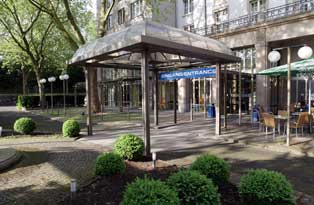
\includegraphics[width=0.25\linewidth]{images/accommodation/auo/bild2.jpg}%
    };
    \node[inner sep=0,outer sep=0,anchor=north west] (img-2) at (main.north east) {%
      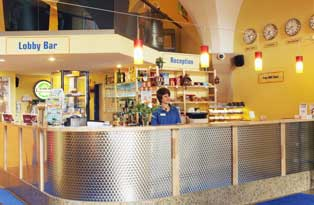
\includegraphics[width=0.25\linewidth]{images/accommodation/auo/bild3.jpg}%
    };
    \node[inner sep=0,outer sep=0,anchor=north west] (img-3) at (img-2.north east) {%
      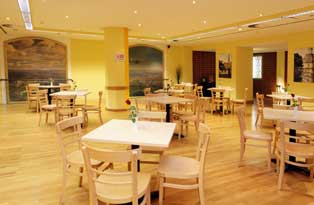
\includegraphics[width=0.25\linewidth]{images/accommodation/auo/bild7.jpg}%
    };
    \node[inner sep=0,outer sep=0,anchor=north west] (img-4) at (img-3.north east) {%
      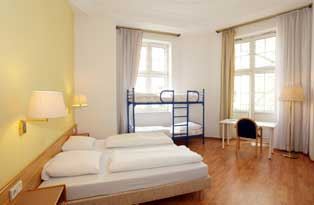
\includegraphics[width=0.25\linewidth]{images/accommodation/auo/bild6.jpg}%
    };
  \end{scope}
  \node[anchor=south west,color=black,xshift=1ex,yshift=1ex] (label) at (main.south west) {\imgtitle{A\&O HOTELS and HOSTELS Holding AG}{A\&O Hostel Karlsruhe}{non-free, permission to use for bid}};
  \begin{scope}[on background layer]
    \node[fit=(label),inner sep=0,outer sep=0,opacity=0.6,fill=white,rounded corners] {};
  \end{scope}
\end{tikzpicture}


\begin{labeling}{\bf Availability}
  \item[\bf Location] Main Station
  \item[\bf Price] single: $\sim\SI{61.30}{/pP}$, 2-3: $\sim\SI{35.30}{/pP}$; 4: $\sim\SI{30.50}{/pP}$
  \item[\bf Breakfast] included, mandatory
  \item[\bf Availability] available
\end{labeling}

This hostel is located right at the main station, which is a little bit off from
the city center. Breakfast is mandatory for group reserverations and the prices
vary quite a lot between the different dates (the estimation is averaged for a
five night stay).

\subsection{Jugendherberge Karlsruhe}

\begin{tikzpicture}
  \begin{scope}[on background layer]
    \node[inner sep=0,outer sep=0] (main) {%
      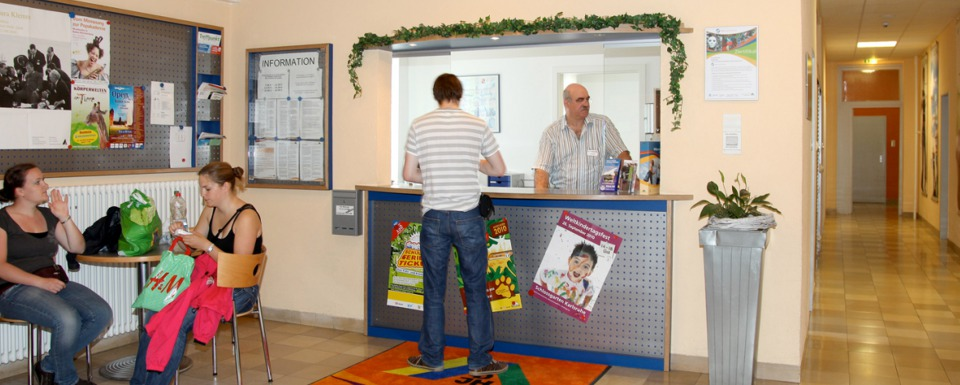
\includegraphics[width=0.5\linewidth]{images/accommodation/jugendherberge/0.jpg}%
    };
    \node[inner sep=0,outer sep=0,anchor=north west] (img-2) at (main.north east) {%
      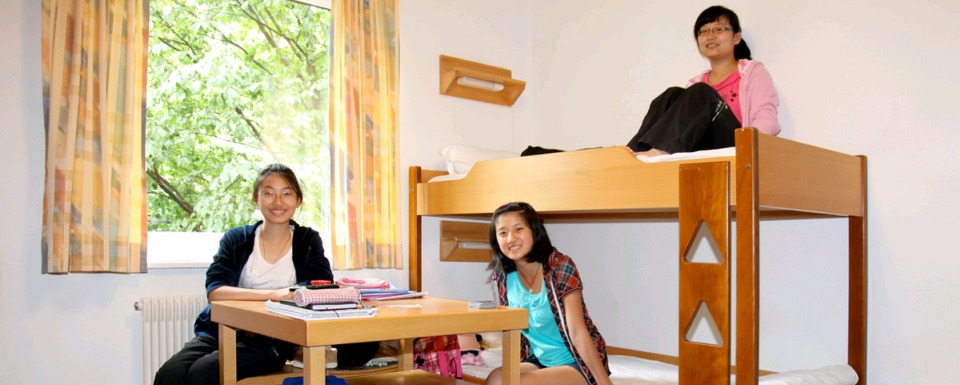
\includegraphics[width=0.5\linewidth]{images/accommodation/jugendherberge/1.jpg}%
    };
  \end{scope}
  \node[anchor=south west,color=black,xshift=1ex,yshift=1ex] (label) at (main.south west) {\imgtitle{}{Jugendherberge Karlsruhe}{non-free, permission to use for bid}};
  \begin{scope}[on background layer]
    \node[fit=(label),inner sep=0,outer sep=0,opacity=0.6,fill=white,rounded corners] {};
  \end{scope}
\end{tikzpicture}

\begin{labeling}{\bf Availability}
  \item[\bf Location] North West of City Center
  \item[\bf Price] $\sim\SI{25}{\euro/{pP}}$
  \item[\bf Breakfast] included, mandatory
  \item[\bf Availability] after 21st August
\end{labeling}

The youth hostel is located to the south west of the city center in the middle
of one of the universities, the Hochschule Karlsruhe. The walk to the
next tram station is about \SI{10}{\minute}. While this location would be
pretty affordable, it is heavily used by groups during the summer, and will
not be available to us from the start of Juli till the 21st of August.

Note that it is mandatory to get half-board or a lunch pack for at least some
of the days. The price mentioned here is an estimation that already includes
the extra costs this incurs.

\subsection{Gästehaus Kaiserpassage}

\begin{tikzpicture}
  \begin{scope}[on background layer]
    \node[inner sep=0,outer sep=0] (main) {%
      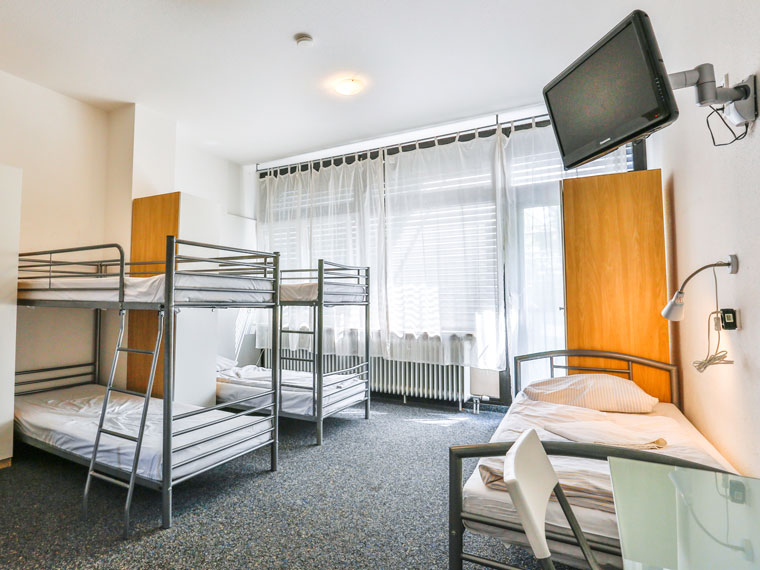
\includegraphics[width=0.5\linewidth]{images/accommodation/kaiserpassage/mehrbettzimmer-2.jpg}%
    };
    \node[inner sep=0,outer sep=0,anchor=north west] (sub-1) at (main.north east) {%
      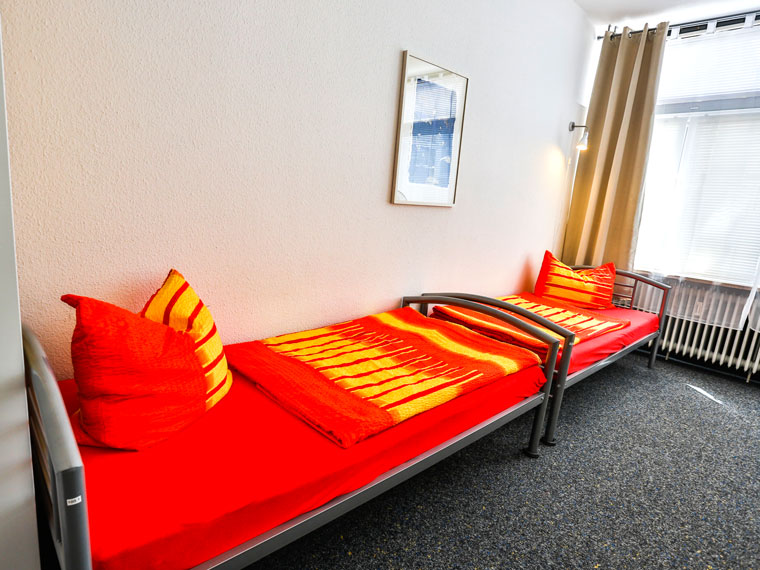
\includegraphics[width=0.25\linewidth]{images/accommodation/kaiserpassage/einzelzimmer.jpg}%
      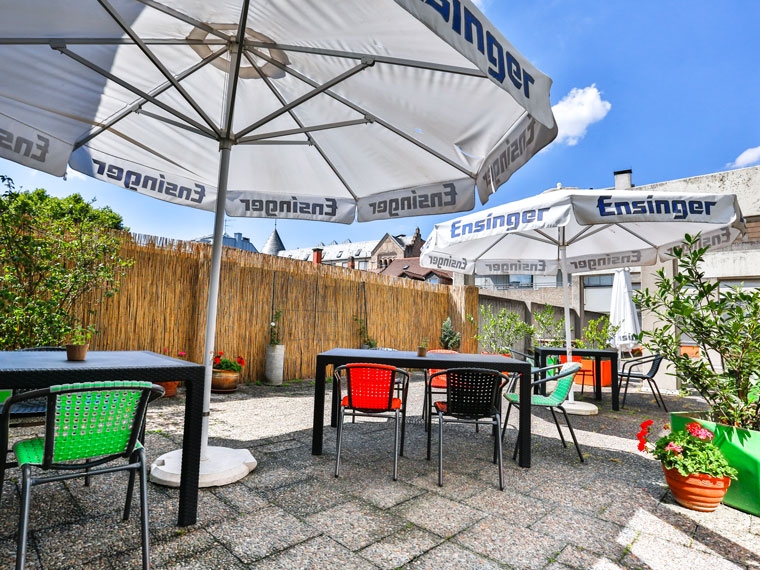
\includegraphics[width=0.25\linewidth]{images/accommodation/kaiserpassage/terasse.jpg}%
    };
    \node[inner sep=0,outer sep=0,anchor=north west] (sub-2) at (sub-1.south west) {%
      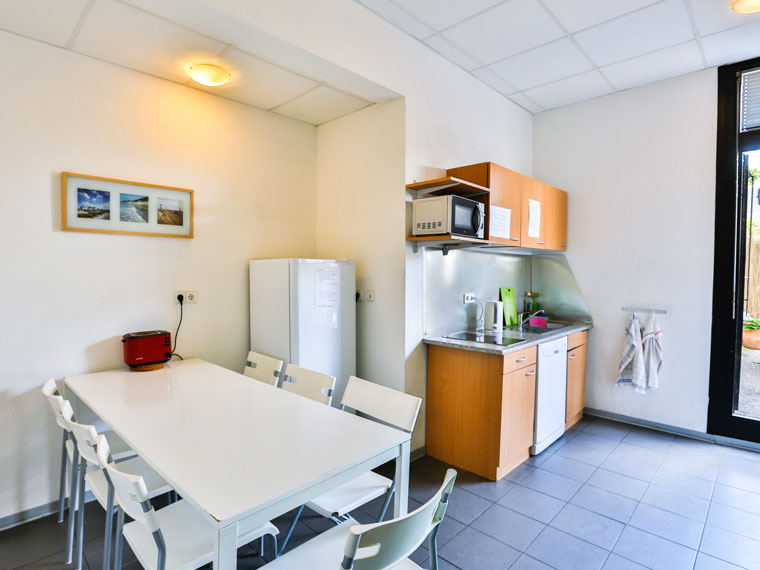
\includegraphics[width=0.25\linewidth]{images/accommodation/kaiserpassage/gemeinschaftskueche.jpg}%
      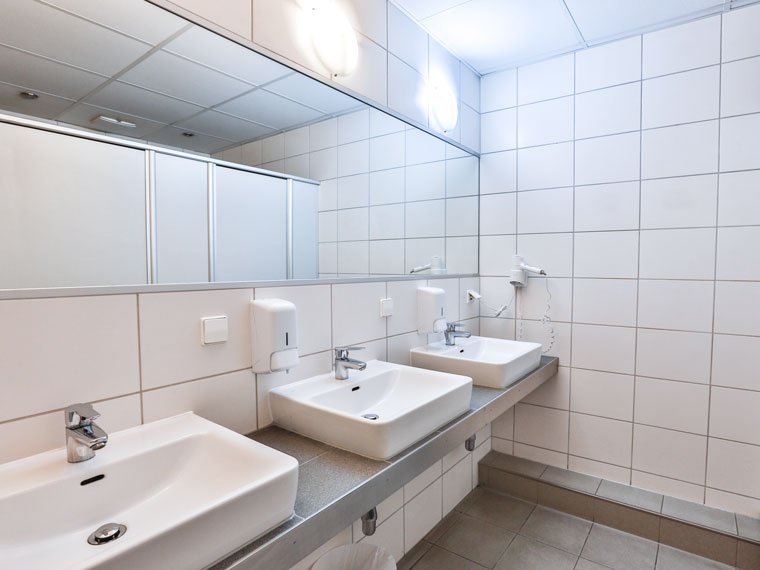
\includegraphics[width=0.25\linewidth]{images/accommodation/kaiserpassage/badezimmer.jpg}%
    };
  \end{scope}
  \node[anchor=south west,color=black,xshift=1ex,yshift=1ex] (label) at (main.south west) {\imgtitle{Gästehaus Kaiserpassage}{Gästehaus Kaiserpassage}{non-free, permission to use for bid}};
  \begin{scope}[on background layer]
    \node[fit=(label),inner sep=0,outer sep=0,opacity=0.6,fill=white,rounded corners] {};
  \end{scope}
\end{tikzpicture}

\begin{labeling}{\bf Availability}
  \item[\bf Location] West of City Center
  \item[\bf Price] \num{20} to \SI{22}{\euro/{pP}} in 4 bed room
  \item[\bf Breakfast] not available
  \item[\bf Availability] available
\end{labeling}

This small hostel is located in the western part of the city center. The hostel
does not offer breakfast or en-suite bathrooms. The hostel offers a shared
kitchen.

\subsection{B\&B Hotels}

\begin{labeling}{\bf Availability}
  \item[\bf Location] Main Station
  \item[\bf Price] \SI{33}{\euro/{pP}} in 2 bed room, \SI{28.70}{\euro/{pP}} in 3 bed room
  \item[\bf Breakfast] \SI{7,50}{\euro/{pP}}
  \item[\bf Availability] available
\end{labeling}

This is a relatively cheap hotel just behind the main station.


\newpage

\section{Dining}

\subsection{Breakfast}
There are little German bakeries all over the city where you can get breakfast (savory or sweet pastries and coffee or tea) for about 4 euros. However, breakfast is included in room fares at the Ibis hotel and A\&O, as well B\&B have common dining rooms and kitchen where everyone can prepare their usual breakfast.
 
\subsection{Lunch}
The university canteen offers meals for about 3 euros. Otherwise, all type of restautrants (kebabs, thai,chinese, italian etc.) are available all over the inner city. On average, one should budget about 6 euros per meal.


\subsection{Dinner}
We intend to organize a picnic in the “Schlosspark” on Tuesday, as well as a BBQ on Friday. For the other evenings, we would suggest to have dinner at one of the three “Hammer” options (Kippe, Emaille, Blue) for under a fiver, including a glass of beer! Of course, other options are available in this city which is known for its student-friendly prices!


As you can see, accessibility of the location, prices of accommodation and meals, as well as the overall concept elaborated by the organizing committee are all speaking in favor of hosting GUADEC in August 2016 in the sunny city of Karlsruhe! We are looking forward to welcoming you!


\section{Team}

The team is currently composed of three people:
Benjamin Berg, Moira Schuler, and Tobias Mueller.

We have commitments from more people both local and remote.
We will need more help, though, and we have already discussed
what the roles and responsibilities are that need to be distributed.

Local GNOME communities are hard to find in Germany, these days,
so there is no local GNOME user group in Karlsruhe.
But there are several IT and IT friendly institutions such as the
the local CCC branch called Entropia, a fablab, and several LUGs.
Some of those have already organised an event like GUADEC and
we hope to make use of their knowledge.

As for the legal structure supporting the event,
we consider founding registered student association at
the university to get hold of the univerity's resources,
but also to tap into the student's pool more easily.
We also consider founding a German non-profit which will reduce
liability for the organisers.


\section{Budget}



\sisetup{
table-figures-integer = 0,
table-figures-decimal = 0,
negative-color=red,
table-text-alignment=right,
table-number-alignment=right,
table-figures-integer=5,
table-figures-decimal=2,
}
 
\begin{tabularx}{\linewidth}{XSSS}
   & {Best Case} & {Expected} & {Worst Case} \\
  \hline\hline
Income \hspace*{1em}  & {} & {} & {}\\
\hspace*{1em} Donations at Registration  & 9000.00 & 5250.00 & 3750.00\\
\hspace*{1em} Sponsorship (via foundation)  & 35000.00 & 32000.00 & 30000.00\\
\hspace*{1em} Sponsorship (local)  & 10000.00 & 5000.00 & 2000.00\\
\hspace*{1em} Merchandise  & 1600.00 & 1300.00 & 1000.00\\[0.5ex]
Expenses \hspace*{1em}  & {} & {} & {}\\
\hspace*{1em} Liability Insurance  & -200.00 & -200.00 & -200.00\\
\hspace*{1em} Lanyards  & 0.00 & 0.00 & 0.00\\
\hspace*{1em} Merchandise  & -800.00 & -800.00 & -800.00\\
\hspace*{1em} Video and Live Streaming\footnote{This assumes the CCC Video Operation Center provides the video and streaming infrastructure.}  & {} & {} & {}\\
\hspace*{1em} \hspace*{1em} Travel and Accomodation & -175.00 & -300.00 & {–}\\
\hspace*{1em} \hspace*{1em} Equipment Insurance & -100.00 & -100.00 & {–}\\
\hspace*{1em} \hspace*{1em} Shipping & {–} & -150.00 & {–}\\
\hspace*{1em} Travel Sponsorship  & -35000.00 & -30000.00 & -30000.00\\
\hspace*{1em} Keynote Speaker Travel  & -3500.00 & -3000.00 & -2500.00\\
\hspace*{1em} Venue  & -2000.00 & -4500.00 & -8000.00\\
\hspace*{1em} Social Events  & {} & {} & {}\\
\hspace*{1em} \hspace*{1em} AKK/Z10 Evening with drinks & -1000.00 & -500.00 & {–}\\
\hspace*{1em} \hspace*{1em} Picnic & -500.00 & -300.00 & {–}\\
\hspace*{1em} \hspace*{1em} Barbecue & -1000.00 & -1000.00 & {–}\\
\hspace*{1em} \hspace*{1em} Football Field Rental & 0.00 & 0.00 & 0.00\\
\hspace*{1em} Misc  & {} & {} & {}\\
\hspace*{1em} \hspace*{1em} Speaker Gifts & -500.00 & -300.00 & -200.00\\
\hspace*{1em} \hspace*{1em} KVV tickets for everyone & -800.00 & -800.00 & {–}\\
\hspace*{1em} \hspace*{1em} Car Rentals & -800.00 & -800.00 & -300.00\\
\hspace*{1em} \hspace*{1em} Coffee Breaks & -300.00 & -300.00 & {–}\\
\hspace*{1em} \hspace*{1em} Admin and Bank & -750.00 & -750.00 & -750.00\\
\hspace*{1em} \hspace*{1em} Speaker/Volunteer Water & -50.00 & -50.00 & -50.00\\[0.5ex]\hline
\bf Sum \hspace*{1em}  & 8125.00 & -300.00 & -6050.00\\
\end{tabularx}

\newpage



%%%%%%%%%%%%%%%%%%%%%%%%

  \section{Images}
  \begin{enumerate}
    \imagecopyrights
  \end{enumerate}

  \section{Licenses}

  \begin{description}
    \item[CC BY-SA 2.0] https://creativecommons.org/licenses/by-sa/2.0/
    \item[CC BY-SA 2.5] https://creativecommons.org/licenses/by-sa/2.5/
  \end{description}

\end{document}

